% !TEX program = xelatex
% =====================================================================
%  持续状态语言模型：固定大小状态能否承载跨上下文信息？
%  （初稿；按《论文大纲-A.md》+《论文大纲-A-第1-3章详细说明-10.9修正.md》结构，
%    数字来自 BSKD 实验包，其中已按 BSKD-修复/说明.md 订正过三处口径）
%
%  编译：xelatex main → bibtex main → xelatex main ×2   （见 如何编译.md）
% =====================================================================
\documentclass[11pt,a4paper]{ctexart}

\usepackage[margin=2.4cm]{geometry}
\usepackage{graphicx}
\usepackage{booktabs}
\usepackage{amsmath,amssymb}
\usepackage{xcolor}
\usepackage[numbers,sort&compress]{natbib}
\usepackage[colorlinks=true,linkcolor=blue!60!black,citecolor=green!45!black,
            urlcolor=blue!60!black]{hyperref}
\usepackage{caption}
\usepackage{placeins}   % FloatBarrier：把浮动体锁在本节内，避免换页时溢到下一节页首
\usepackage{tabularx}   % 表格自动换行，防内容冲出纸边
\usepackage{float}      % [H]：强制浮动体原地，用于节内首个浮动体（否则会被拉到本页顶部压住大标题）
\usepackage{longtable}  % 超过一页高的大表（tab:config）用，可原地起排并自然跨页
\captionsetup{font=small,labelfont=bf}
\graphicspath{{figs/}}

% ---- 草稿期标记 ----
\newcommand{\pending}[1]{\textcolor{red}{\textbf{[待补：#1]}}}
\newcommand{\draftnote}[1]{\textcolor{blue!70!black}{\small #1}}
\newcommand{\bits}{\ensuremath{\,\mathrm{bit/byte}}}
\newcommand{\nats}{\ensuremath{\,\mathrm{nat}}}

% ---- 版式（2026-10-23）：每个大标题另起一页，标题位于页首 ----
% 中标题/小标题不拆页。FloatBarrier 先把上一节遗留的浮动图表锁在本节内，
% 再换页，避免图表溢到新节页首把标题顶下去。
\let\origsection\section
\renewcommand{\section}{\FloatBarrier\clearpage\origsection}

\title{\textbf{State Is All You Need}\\[4pt]
\large ——以中型 byte 级有状态语言模型 Gridman/Ouro 为对象的实证研究（初稿）}
\author{作者列表 \pending{待填}\\[2pt]
\small 单位 / 通讯作者 \pending{待填}}
\date{\today}

\begin{document}
\maketitle

\begin{center}
\fbox{\parbox{0.94\linewidth}{\small
\textbf{本文状态（草稿，投稿前请先读这一段）}
\begin{itemize}\itemsep2pt
\item 所有数字来自\textbf{单一检查点}：\texttt{gridman\_medium\_v\_0d3\_pretrain}，step 144000/705600，即训练进度\textbf{约 20\%}。
      模型行为描述以现行实现 \textbf{v\_0d4} 为准（memory 改为序列级私有槽位，两版存档不兼容；
      $\mathrm{batch}=1$ 推理两版逐位对应，见 \S\ref{sec:model} 表 \ref{tab:version}）。
      因此本文只做\textbf{条件间的相对比较}，任何绝对值（如 1.08\bits）都\textbf{不可}与外部模型对照。加验证集、训完 medium、
      补同预算基线（\S\ref{sec:b3}）之前，本稿不可当作最终结果。
\item 已完成并可报：A1/A2/A3/A5/A6（第 \ref{sec:s1} 章）、B1-lite/B2/B2-freeze（第 \ref{sec:s2} 章）、
      以及稳定性与状态性质（附录 \ref{app:cline}、\ref{app:dline}）。
\item \textbf{未完成}：A4（状态错配）、B3（等效滑窗基线）、B4（needle 预实验）、F 线（重训类）。
      正文中未完成处一律以 \pending{} 标出，不预留空节。
\item \textbf{已作废}：受控遗忘曲线（C1）因实现缺陷（答案位置整体偏移，实际在测补白字节）作废，
      不从正文引用；完整说明见附录 \ref{app:c1}。
\end{itemize}}}
\end{center}

\section*{摘要}
\addcontentsline{toc}{section}{摘要}

标准语言模型把历史信息的载体固定在上下文窗口里：窗口内的 token 可被注意力直接访问，窗口之外的历史要么不可见，
要么必须以随长度增长的成本重新写回窗口。持续状态是另一种载体——一段形状固定的张量，跨上下文持续存在，
在前向过程中被反复读写，其容量\textbf{不随历史长度增长}。本文把「固定大小的持续状态能承载多少跨上下文信息」
作为可以用实验正面验证的经验问题，在一个 437.8M 参数的中型 byte 级有状态语言模型（Gridman/Ouro medium）上做系统测量。
评测只使用训练到 20\%（step 144000/705600）的单一检查点，全程 teacher-forced、不做任何重训，
并把操纵旋钮全部落在架构暴露的状态接口上：\textbf{起点状态}（热启动 / 空白）、\textbf{读写路径}（commit / lock）、
\textbf{组件手术}（重置 / 冻结）。

主要结果：（1）状态的跨上下文携带\textbf{成立}：在同一计分窗口下，热启动起点比失忆起点低
$3.73\bits$（$1.59$ 对 $5.32$），且该差距在窗口内不收敛；锁定跨 patch 写入的代价是
$+1.00\pm0.09\bits$，并在上下文增长时\textbf{累积}（后段 $0.77$ 对前段 $0.58\nats$）；
跨文档边界重置造成 $+0.45\nats$ 的冲击，但中位数 1 个 patch 即自愈。
（2）组件归因给出一个反直觉的结论：自然文本上的跨 patch 适应\textbf{几乎全部由块级循环状态（recurrent c\_state）承担}——
冻结它等价于冻结全部写入（$+1.02$ 对 $+1.03\bits$），而冻结 delta 规则矩阵记忆（memory）的写入代价
$\approx 0$（$-0.0005\bits$）；矩阵记忆的价值不在增量适应，而在\textbf{读取训练稳态先验}。
（3）有效上下文\textbf{有限}：自然重复带来的复现增益集中在 $1$k token 以内（$+0.084\nats$），
$4$k 之外衰减到零甚至转负；冻结 recurrent 会精确抹平该增益。这修正了「固定状态长程记忆 $\ge 256$K 不衰减」的初步结论
（该结论源于一次分桶实现的缺陷，已作废重测）。
（4）永续性侧的证据是正面的：$96$KB / $512$KB 连续写入下状态范数有界缓增
（memory $\times1.02/\times1.13$、MTM $\times1.02/\times1.07$，STM/queue 恒定），
重置频率扫描单调（$512\text{tok}\to\infty$：$1.215\to1.039\bits$），未见噪声累积。
（5）一条必须写进评测协议的警示：热启动状态里含有\textbf{逐样本的训练痕迹}——
在训练消费区文本上热启动的优势比未消费文本低 $0.35\pm0.20\bits$，且这一成分几乎全部由状态承载
（去掉热启动后该差距消失：$+0.36\pm0.83$），因此主表必须\textbf{双报起步状态}。

结论：固定大小的持续状态在这个规模上确实承载了可测的跨上下文信息与稳定的长时写入能力，
但其\textbf{有效记忆距离约为 $1$–$4$k token}，与「永续上下文」的强主张尚有量级差距；
且承载者主要是循环状态而非参数化矩阵记忆。本文同时给出未完成项（状态错配、等效滑窗基线、精确检索预实验）
与已作废实验（受控遗忘曲线）的完整说明。

\vspace{0.6em}
\noindent\textbf{关键词：有状态语言模型；持续状态；固定大小记忆；delta 规则快权重；有效上下文；
teacher-forced bits/byte；评测协议}

\vspace{1.0em}
\section*{Abstract}
\addcontentsline{toc}{section}{Abstract}

Standard language models carry history in the context window: tokens inside the window are directly
attended to, while history outside it is either invisible or must be replayed at a cost that grows with
length. A \emph{persistent state} is an alternative carrier---a fixed-shape tensor that exists across
contexts, is read and written at every forward pass, and whose capacity does not grow with history
length. We turn ``how much cross-context information can a fixed-size persistent state carry'' into an
empirical question and measure it on a 437.8M-parameter byte-level stateful LM (Gridman/Ouro medium),
using a single checkpoint at $20\%$ of training (step 144000/705600), teacher-forced evaluation, and no
retraining. All control knobs are architecture-exposed state operations: the \emph{starting state}
(hot start vs.\ blank), the \emph{read/write path} (commit vs.\ lock), and \emph{component surgery}
(reset / freeze). We find that (i) cross-context carriage holds---on a common scoring window the hot
start beats a blank start by $3.73$\,bits/byte ($1.59$ vs.\ $5.32$) with no convergence trend, and
locking cross-patch writes costs $+1.00\pm0.09$\,bits/byte, growing with context length;
(ii) cross-patch adaptation is almost entirely carried by the block-level recurrent state---freezing it
costs as much as locking all writes ($+1.02$ vs.\ $+1.03$\,bits/byte), while freezing the global
delta-rule matrix memory is free ($-0.0005$); (iii) the effective repetition memory is limited to about
$1$--$4$k tokens; and (iv) the hot-start state contains sample-level training traces, so any main table
must report both starting states.

\vspace{0.6em}
\noindent\textbf{Keywords:} stateful language model; persistent state; fixed-size memory; delta-rule fast
weights; effective context; teacher-forced bits/byte


\section{绪论}\label{sec:intro}

\subsection{背景：语言模型的上下文与状态}\label{sec:bg}

\textbf{先说循环网络这一路。}LSTM/GRU 及其变体\citep{hochreiter1997lstm,cho2014gru}
是最早把「固定大小的状态」写进架构的一路：
一步一递归，历史被压缩进一个形状固定的隐状态。这个想法本身是对的，但它没有走到今天，原因有两条。
其一，\textbf{状态太小}：一般只有 KB 到 MB 量级，容量撑不住长历史；其二，\textbf{效果不好}：
长程依赖学不动、训练也不稳定，于是被「更大的窗口 + 注意力」一路取代。
所以要把问题评准——症结不在「固定状态」这个想法，而在\textbf{当时的状态不够大、写入方式不够好}。
本文接下来做的事，就是把状态放大：我们研究的模型（Gridman/Ouro medium）仅 delta 规则矩阵记忆一项就有
$12{,}954{,}624$ 个 fp32 元素（约 $49.4$\,MiB），推理时 batch$=1$ 的四件套状态切片合计
$14{,}072{,}832$ 个 fp32 元素（约 $53.7$\,MiB：memory $49.4$ $+$ MTM $4.0$ $+$ queue $0.25$ $+$ recurrent $0.016$），
比典型 RNN 状态高出两个到四个数量级。

\textbf{既有架构只有一种信息载体：上下文窗口。}每一步预测都通过注意力读取窗口内所有 token；
窗口之外的历史模型完全看不见——除非把它重新写回窗口（重放），而重放的成本随长度增长
（注意力计算与显存都随长度线性膨胀）\citep{vaswani2017attention,dao2022flashattention,pope2023efficient}。
窗口越开越大是一条路\citep{beltagy2020longformer,ding2023longnet}，但它改变的是「一次能看多少」，
不是「能带多少」。

\textbf{持续状态是另一种载体。}一段形状固定的张量，跨上下文持续存在，在每次前向中被读写，
其容量\textbf{不随历史长度增长}：喂给它 1 千字节还是 100 万字节，状态大小不变。
窗口用「更大」换「记得更多」，状态用「固定」换「持续」——两者的张力正是本文的问题：
固定大小的状态到底能承担多少跨上下文的信息传递？这是一个可以用实验正面验证、给出定量结论的经验问题，
而不是「架构看起来很优雅」式的主张。

\textbf{全文围绕两点：}①\textbf{把状态做大}（scaling up）；
②\textbf{大状态带来的持续学习}——状态跨上下文持续被写入，模型在「读」的过程中仍在改变自己的行为，
而不是读完即定。逻辑链全文固定为：\emph{以前 RNN 效果不好 $\to$ 本文把状态放大 $\to$ 更大的状态带来持续学习。}

\subsection{问题：固定大小的持续状态能否承载跨上下文信息}\label{sec:problem}

\textbf{形式化。}一次前向写成
\begin{equation}
\mathrm{logits},\; s' = f(x, s; \mathit{lock}),
\label{eq:forward}
\end{equation}
其中 $x$ 是当前输入（本文实现中为一个 64 字节的 patch），$s$ 是状态——
\textbf{形状固定，与已处理的历史长度无关}，这就是「固定大小」的字面含义；$s'$ 是写入后的新状态；
$\mathit{lock}$ 是布尔开关，决定这一步 $s$ 是否接受新写入（$\mathit{lock}=\mathrm{true}$ 时状态只读，见 \S\ref{sec:model-io}）。
上下文的延续由 $s' = f(x,s)$ 在 patch 之间递归传递，不依赖 KV cache 的累积。

\textbf{两个待验证的子问题。}它们是本文的两条主张，第 \ref{sec:s1}、\ref{sec:s2} 章分别正面验证：

\begin{itemize}\itemsep4pt
\item \textbf{S1：状态是否持续携带跨上下文信息？}
\emph{成立条件}：\textbf{热启动显著优于空白}、\textbf{正常写入显著优于 $\mathit{lock}$}。
只有当前者成立，才说明状态里带着信息；只有当后者成立，才说明「往状态里写」这件事有因果贡献。
两条同时满足，S1 成立。
\begin{itemize}\itemsep2pt
\item \textbf{热启动（hot start）}：评测起点用训练收敛时保存的稳态状态快照（\S\ref{sec:train}），
      相当于「模型带着训练结束时的记忆来考试」。
\item \textbf{空白（blank）}：评测起点用全初始状态（恒等 memory + 零 recurrent/queue/MTM），
      相当于「模型失忆后开始读」。
\item \textbf{$\mathit{lock}$}：前向过程中状态只读不写——这段上下文的信息\textbf{不许}进入状态；
      它与「正常（commit）」构成一对受控对照，隔离出「写入」的因果贡献。
\end{itemize}
\item \textbf{S2：固定状态的有效上下文窗口有多大？}
\emph{成立条件}：\textbf{有效窗口显著大于 0}——固定状态在损失上确实等效于一段非零的滑动窗口。
\textbf{有效窗口}不是架构参数而是测出来的等效值\pending{测量方法见 \S\ref{sec:b3}，需滑窗基线}。
\end{itemize}

S1 问「有没有」（定性），S2 问「有多少」（定量）。第 \ref{sec:discussion} 章的汇总表把这两问与第 \ref{sec:s1}、\ref{sec:s2} 章的判定句直接对上。

\subsection{本文贡献}\label{sec:contrib}

\textbf{主线句}：以前 RNN 效果不好，是因为状态太小；本文把状态放大，大状态让「跨上下文携带信息」成立，
并进一步带来持续学习。三条贡献分别是这条链上的三段证据。

\textbf{贡献一：起点状态的系统消融结论（回答 S1，第 \ref{sec:s1} 章）。}\
五组对照——热启动 vs 空白（A1）、写入 vs $\mathit{lock}$（A2）、跨文档边界连续 vs 重置（A3）、
状态错配（A4）、组件级归因（A5/A6）——每组预先写明「状态在携带信息时结果应该长这样」的成立预期，
合起来逐条判定状态是否真在携带信息。这是「状态放大了，但里面到底有没有东西」的直接回答。
本文在该簇上的实测结论是：S1 \textbf{成立}，且携带者主要是块级循环状态（\S\ref{sec:s1-attr}）。

\textbf{贡献二：固定大小状态的有效窗口测量（回答 S2，第 \ref{sec:s2} 章）。}\
三把尺交叉定位：位置衰减（长文档上损失随位置怎么走，B1）、重复距离（自然重复内容隔多远还记着，B2）、
等效滑窗（把状态折算成一个窗口宽度数字，B3）。本文已完成前两把尺，第三把尺与精确检索预实验（B4）未完成，
如实标注。结论是\textbf{有效记忆距离约 $1$–$4$k token}：S2 的「显著大于 0」成立，
但远未达到「永续上下文」量级。

\textbf{贡献三：持续状态与有状态架构（第 \ref{sec:model} 章）。}\
架构层面的贡献有两层含义，这里给出的是\textbf{状态在前}的表述：
①\textbf{状态是微观实现、可以显式调整}——它可以整体读出、冻结（$\mathit{lock}$）、置换（重置/换入其他状态），
所以评测旋钮直接落在架构接口上，而不是像无状态模型那样只能从外部改提示词、改窗口；
②\textbf{记忆是宏观体现、可以多方面量度}——记忆不是外挂模块，就是四件套状态
（memory / recurrent / queue / MTM，见 \S\ref{sec:model-state}）在跨上下文尺度上表现出来的能力；
\textbf{持续学习是它在时间维度上的表现}——状态持续被写入，行为随之改变。

\draftnote{说明：原大纲把「teacher-forced bits/byte 评测协议」列为贡献之一，本稿按要求删除——
协议是支撑贡献一、二的手段，不单列为贡献；协议本身在第 \ref{sec:protocol} 章完整定义。}

\textbf{本文材料边界。}本文所报实验全部基于\textbf{单一检查点}（step 144000/705600，约 20\% 训练进度）的推理评测，
不做任何重训；已完成 A1–A3、A5、A6、B2 及其组件归因、外加稳定性（E 线）、
热启动记忆的领域分解与成员推断（D 线）、前向学习（G 线）；
未完成 A4、B3、B4、F 线（需重训）；受控遗忘曲线（C1）因实现缺陷作废，完整说明见附录 \ref{app:c1}。

\section{相关工作}\label{sec:related}

\subsection{持续状态架构：状态与记忆}\label{sec:related-state}

本节把状态与记忆分开讲，因为两者是\textbf{实现与体现}的关系，不是并列的两个东西：
\textbf{状态实现记忆}——状态是前向过程中每一步实际读写的张量对象（实现层）；
\textbf{记忆是状态的宏观体现}——站在跨上下文的尺度看，「模型记得之前读过什么」这个能力，
就是状态被反复读写的累积效果。所以 \S\ref{sec:related-state} 先讲状态（微观、实现），再讲记忆（宏观、能力）。

\subsubsection{状态：架构的实现层}\label{sec:related-state-impl}

\textbf{定义。}状态是模型内部一组形状固定的张量对象，随前向逐步读写，不随历史长度增长。

\textbf{与 RNN 的关系：思想类似，实现差异很大。}两者都用固定大小的循环状态承载历史，
但本文研究的架构在四点上都不同于 RNN：
（i）不是单一隐向量的逐步递归，而是\textbf{四件套按时间尺度分工}
（delta 规则矩阵 memory + 逐层 c\_state + 滚动 queue + 中期 MTM，见 \S\ref{sec:model-state}）；
（ii）memory 的写入用 \textbf{delta 规则快权重}
\citep{schmidhuber1992learning,schlag2021linear,sun2023retnet,yang2024deltanet}，
而不是 RNN 的门控线性更新；
（iii）\textbf{规模不同}：RNN 的状态一般只有 KB--MB 级，本文的状态高出若干数量级（\S\ref{sec:bg}）——
「把容量做大」在参数规模上已有系统性的经验规律\citep{kaplan2020scaling}，
把同样的思路用在\textbf{状态}上正是本文的出发点；
（iv）\textbf{训练方式不同}：RNN/RWKV 训练时状态从零初始化、一批读完即清零，
单个状态最多跨一个样本（例如 2000 token）；本文的模型不按批次清空，
上一批结束时的状态直接续进下一批，整条训练流是一条全局连续的流（\S\ref{sec:train}）。
最后、也是最关键的一点：状态被设计成\textbf{可以整体读出、冻结、置换的显式对象}——
RNN 的隐状态没有对评测暴露这样的接口。

\textbf{与测试时训练/记忆模块一类工作的关系。}把「记忆」做成层内的可学习结构并非新想法：
快权重\citep{schmidhuber1992learning,ba2016using}、TTT\citep{sun2024ttt}、
Titans\citep{behrouz2025titans} 都让模型在前向中写入某种内部状态；
线性注意力/状态空间模型\citep{katharopoulos2020transformers,gu2023mamba,peng2023rwkv}
则把递归写成可并行扫描的形式。本文研究的架构在「读取用 delta 规则、写入用误差驱动外积」这一点上与它们同源，
区别在把该规则\textbf{嵌入到每一处线性投影}而不是只放在注意力位置，并把状态拆成四个时间尺度、
以显式对象的形式暴露给评测。本文的实验关心的不是「谁更强」，而是\textbf{这个状态里到底有什么、能带多远}。

\subsubsection{记忆：状态的宏观体现}\label{sec:related-mem}

\textbf{定义。}记忆 $=$ 状态在跨上下文信息传递上表现出的宏观能力；它与 \S\ref{sec:related-state-impl} 的状态
是同一个东西的两个观察尺度，\textbf{不是并列的两个模块}。

\textbf{与记忆增强路线的对照。}既有工作大多把记忆放在架构之外：外部记忆库或检索式增强
\citep{grave2017improving,lewis2020rag}从外部语料/存储里捞回信息；
滑窗或长窗口\citep{beltagy2020longformer,ding2023longnet}把记忆放进更长的窗口；
循环记忆 token\citep{bulatov2022recurrent}把记忆放在一串可训练槽里并通过反向传播更新。
这些路线的共同点是记忆\textbf{不在模型状态里}——要么在外存，要么在窗口，要么在参数。
本文研究的记忆完全由持续状态承载：不依赖重放、不借助外部存储、不靠额外参数。

\textbf{从「记忆全部落在持续状态上」到持续学习。}记忆既然全部落在持续状态上，
而状态在每次前向都被写入，那么模型在阅读过程中仍在改变自己的行为——这就是持续学习：
学习不只发生在训练时，也发生在推理的前向之中（与上下文内学习这一现象相关但并不相同：
ICL 是「看示例就会」\citep{brown2020gpt3,olsson2022induction,chan2022data}，
本文关心的是「读着读着状态变了、行为随之变了」）。这与「损失可塑性」\citep{dohare2024loss}是同一个问题的两个方向：既有工作关心\textbf{反复训练时会不会变坏}，
本文关心\textbf{一次前向流之内，行为会不会变好、变多少}。
可验证的含义是：在分布内/分布外的文本流上，模型的有效行为会随前向推进而改变——
本文用 A2/A6（写入的因果贡献与组件归因）、G 线（合成任务上的学习曲线）
以及 D 线（热启动记忆的领域特异性）三组证据来量这个「读着读着变了多少」。

\subsection{长上下文评测方法}\label{sec:related-eval}

\textbf{needle（needle-in-a-haystack）}\citep{kamradt2023needle}：
在长文本中埋入一条「针」，读完后提问，测模型能否精确检索。它是二值的（对/错），测的是\emph{检索}能力。
本文只把它作为边界预实验（\S\ref{sec:b4}）——固定大小状态的强项未必是精确定位，
所以如实限定 claim 边界，失败也写进 Limitations。

\textbf{滑窗基线}：用一个固定窗口宽度 $W$ 的滑动窗口模型作参照，
看固定状态的逐位置损失落在哪个 $W$ 上，从而把「状态记了多少」折算成一个直观数字「等效窗口宽度」（\S\ref{sec:b3}）。

\textbf{per-position 分析}：不只报一个总分，而是把损失\textbf{按位置逐点对齐}报告随位置的走向。
总分会掩盖结构：衰减形状、边界冲击、恢复长度只有逐位置曲线才看得见。
本文的位置衰减曲线（\S\ref{sec:b1}）与边界恢复曲线（\S\ref{sec:a3}）都属于这一口径。

\textbf{既有方法与本文的接点。}既有方法测的是「上下文（窗口）能看多远」，
本文测的是「固定状态能带多远」；两者底层指标口径相同（teacher-forced 逐位置损失），
因此结果可以互相对照——这也意味着本文的评测协议必须把「起点状态」写清楚（\S\ref{sec:cond}），
否则对照不成立。

\subsection{创新点总结}\label{sec:related-innovation}

\textbf{vs RNN}（\S\ref{sec:related-state-impl}）：思想类似——都用固定大小的循环状态承载历史；
但实现差异很大——不是单一隐向量的逐步递归，而是四件套按时间尺度分工，memory 用 delta 规则快权重写入；
规模上 RNN 状态只有 KB--MB 级，本文的状态高出若干数量级；训练方式上 RNN/RWKV 每批清零、
本文状态跨批次连续（\S\ref{sec:train}）；最关键的差别是状态被设计成\textbf{可整体读出、冻结、置换的显式对象}。

\textbf{vs 记忆增强路线 / 长上下文}（\S\ref{sec:related-mem}）：
既有工作把记忆放在架构之外——外部记忆库、检索增强、或单纯堆长上下文窗口；
本文的记忆完全由持续状态承载，不重放、不外挂，并在持续写入中得到持续学习。
一句话：别人的记忆在状态之外，本文的记忆就是状态在跨上下文尺度上的宏观体现。

\textbf{vs 既有评测方法}（\S\ref{sec:related-eval}）：
needle、滑窗基线、per-position 各自测的是「窗口能看多远」；本文沿用同一底层口径
（teacher-forced 逐位置损失，结果可相互对照），但把操纵旋钮从「改窗口」换成「动状态」——
热启动 / $\mathit{lock}$ / 重置 / 冻结全部落在状态接口上。

\textbf{vs 传统无状态架构}：状态即 KV cache，随输入即生即灭、不可操纵，
推理期不会因为读了新内容而改变自己；本文的状态是显式对象，可整体读出、冻结、置换，
且持续写入带来持续学习。这正对应贡献三的第一层表述——\textbf{状态是微观实现，可以显式调整}。

\textbf{汇总（围绕核心两点）}：本文的创新点 = ①\textbf{状态放大}（scaling up，
状态参数量相对 RNN 高出若干数量级，容量差两个到四个数量级）；
②\textbf{持续学习}（状态跨上下文持续写入，模型在前向中仍在改变自己的行为）。
这两点的可评测性由架构保证——状态是显式对象（可动），记忆可由位置衰减 / 重复距离 / 等效窗口三把尺量（可测）。

\section{模型：持续状态架构}\label{sec:model}

\subsection{整体结构（byte 级语言模型 + 有状态核心）}\label{sec:model-overall}

模型由两部分组成。

\textbf{（1）byte 级语言模型。}分词单位是\textbf{字节}而不是词：ByteTokenizer 直接以 UTF-8 字节为 token，
词表大小 300（256 个字节值 $+$ \texttt{pad}=256 $+$ \texttt{eos}=257）。
好处是不存在词表外的「词」，任何文本都能无损进出；损失以 \textbf{bits/byte} 计，
跨语言、跨编码格式可比——这就是主指标口径的来源（\S\ref{sec:metric}）。

\textbf{（2）有状态核心。}一次前向吃一个 64 字节的 patch（记 $B=64$）：
\begin{equation}
\mathrm{logits},\; \mathrm{state} = \mathrm{model}(x,\ \mathrm{state},\ \mathit{lock\_mem}),
\qquad x \in \mathbb{Z}_B^{1\times 64},
\label{eq:model-call}
\end{equation}
上下文的延续不靠 KV cache 累积，靠 $s' = f(x,s)$ 在 patch 之间递归传递（式 \eqref{eq:forward}）。
注意力只在\textbf{当前 patch 片内}做局部混合，跨 patch 的历史一律由状态携带——
这就是「有状态」的准确含义：历史信息的唯一通道是状态。

图 \ref{fig:arch} 给出整体结构与原语的对应关系。正式配置为 \texttt{GRIDMAN\_MEDIUM}：
\texttt{embed\_dim}=1024、\texttt{blocks}=3（对应 4 个 \texttt{c\_state}）、
\texttt{patch\_size}=64，模型参数 437.8M\footnote{配置与参数量引自团队内部文档《论文大纲-B》第 0 章与配图；
代码事实对应实现仓 \texttt{zhihumomo/ouro-research}。}。

\textbf{实现版本声明（重要）。}本文所有实验数字来自 \texttt{v\_0d3} 检查点；
模型行为的描述以 \texttt{v\_0d4} 实现（2026-10-18 更新）为准。两版差异集中在
\texttt{memory} 的作用域与训练配置，见表 \ref{tab:version}。
差异不影响本文的推理侧结论：所有评测都在 $\mathrm{batch}=1$ 上进行，
v\_0d4 的序列级记忆在 $\mathrm{batch}=1$ 时读写单个槽位，与 v\_0d3 的
\texttt{[1,\ldots]} 布局逐位对应（\S\ref{sec:train}）。

\begin{table}[H]
\centering
\caption{实现版本差异（v\_0d3 $\to$ v\_0d4）。本文检查点由 v\_0d3 训练产生；行为描述以 v\_0d4 为准。}
\label{tab:version}
\footnotesize
\begin{tabularx}{\linewidth}{@{}l X X@{}}
\toprule
项 & v\_0d3（本文检查点） & v\_0d4（现行实现） \\
\midrule
\texttt{memory} 作用域 & 跨样本共享（形状 $[1,\ldots]$） & \textbf{序列级私有槽位}（$[\mathrm{cap},\ldots]$，$\mathrm{cap}=\mathrm{max\_batch}$） \\
提交规则 & 跨 batch 求均值 & \textbf{无跨流平均}——序列间零泄漏 \\
跨卡同步 & 每 patch \texttt{all\_reduce} 均值 & \textbf{已删除}，记忆 rank 私有不通信 \\
写入门控偏置初始化 & $-6.0$ & $-\ln 63\approx-4.14$（对齐 $4096$-token 队列视界） \\
MEDIUM \texttt{chunk\_size} / \texttt{bptt} & $192$ / $4$ & $1$ / $16$ \\
存档格式 & \texttt{global\_memory} 顶层字段 & memory 移入 per-rank runtime\_states，\textbf{与 v\_0d3 存档不兼容} \\
\bottomrule
\end{tabularx}
\end{table}

\begin{figure}[t]
\centering
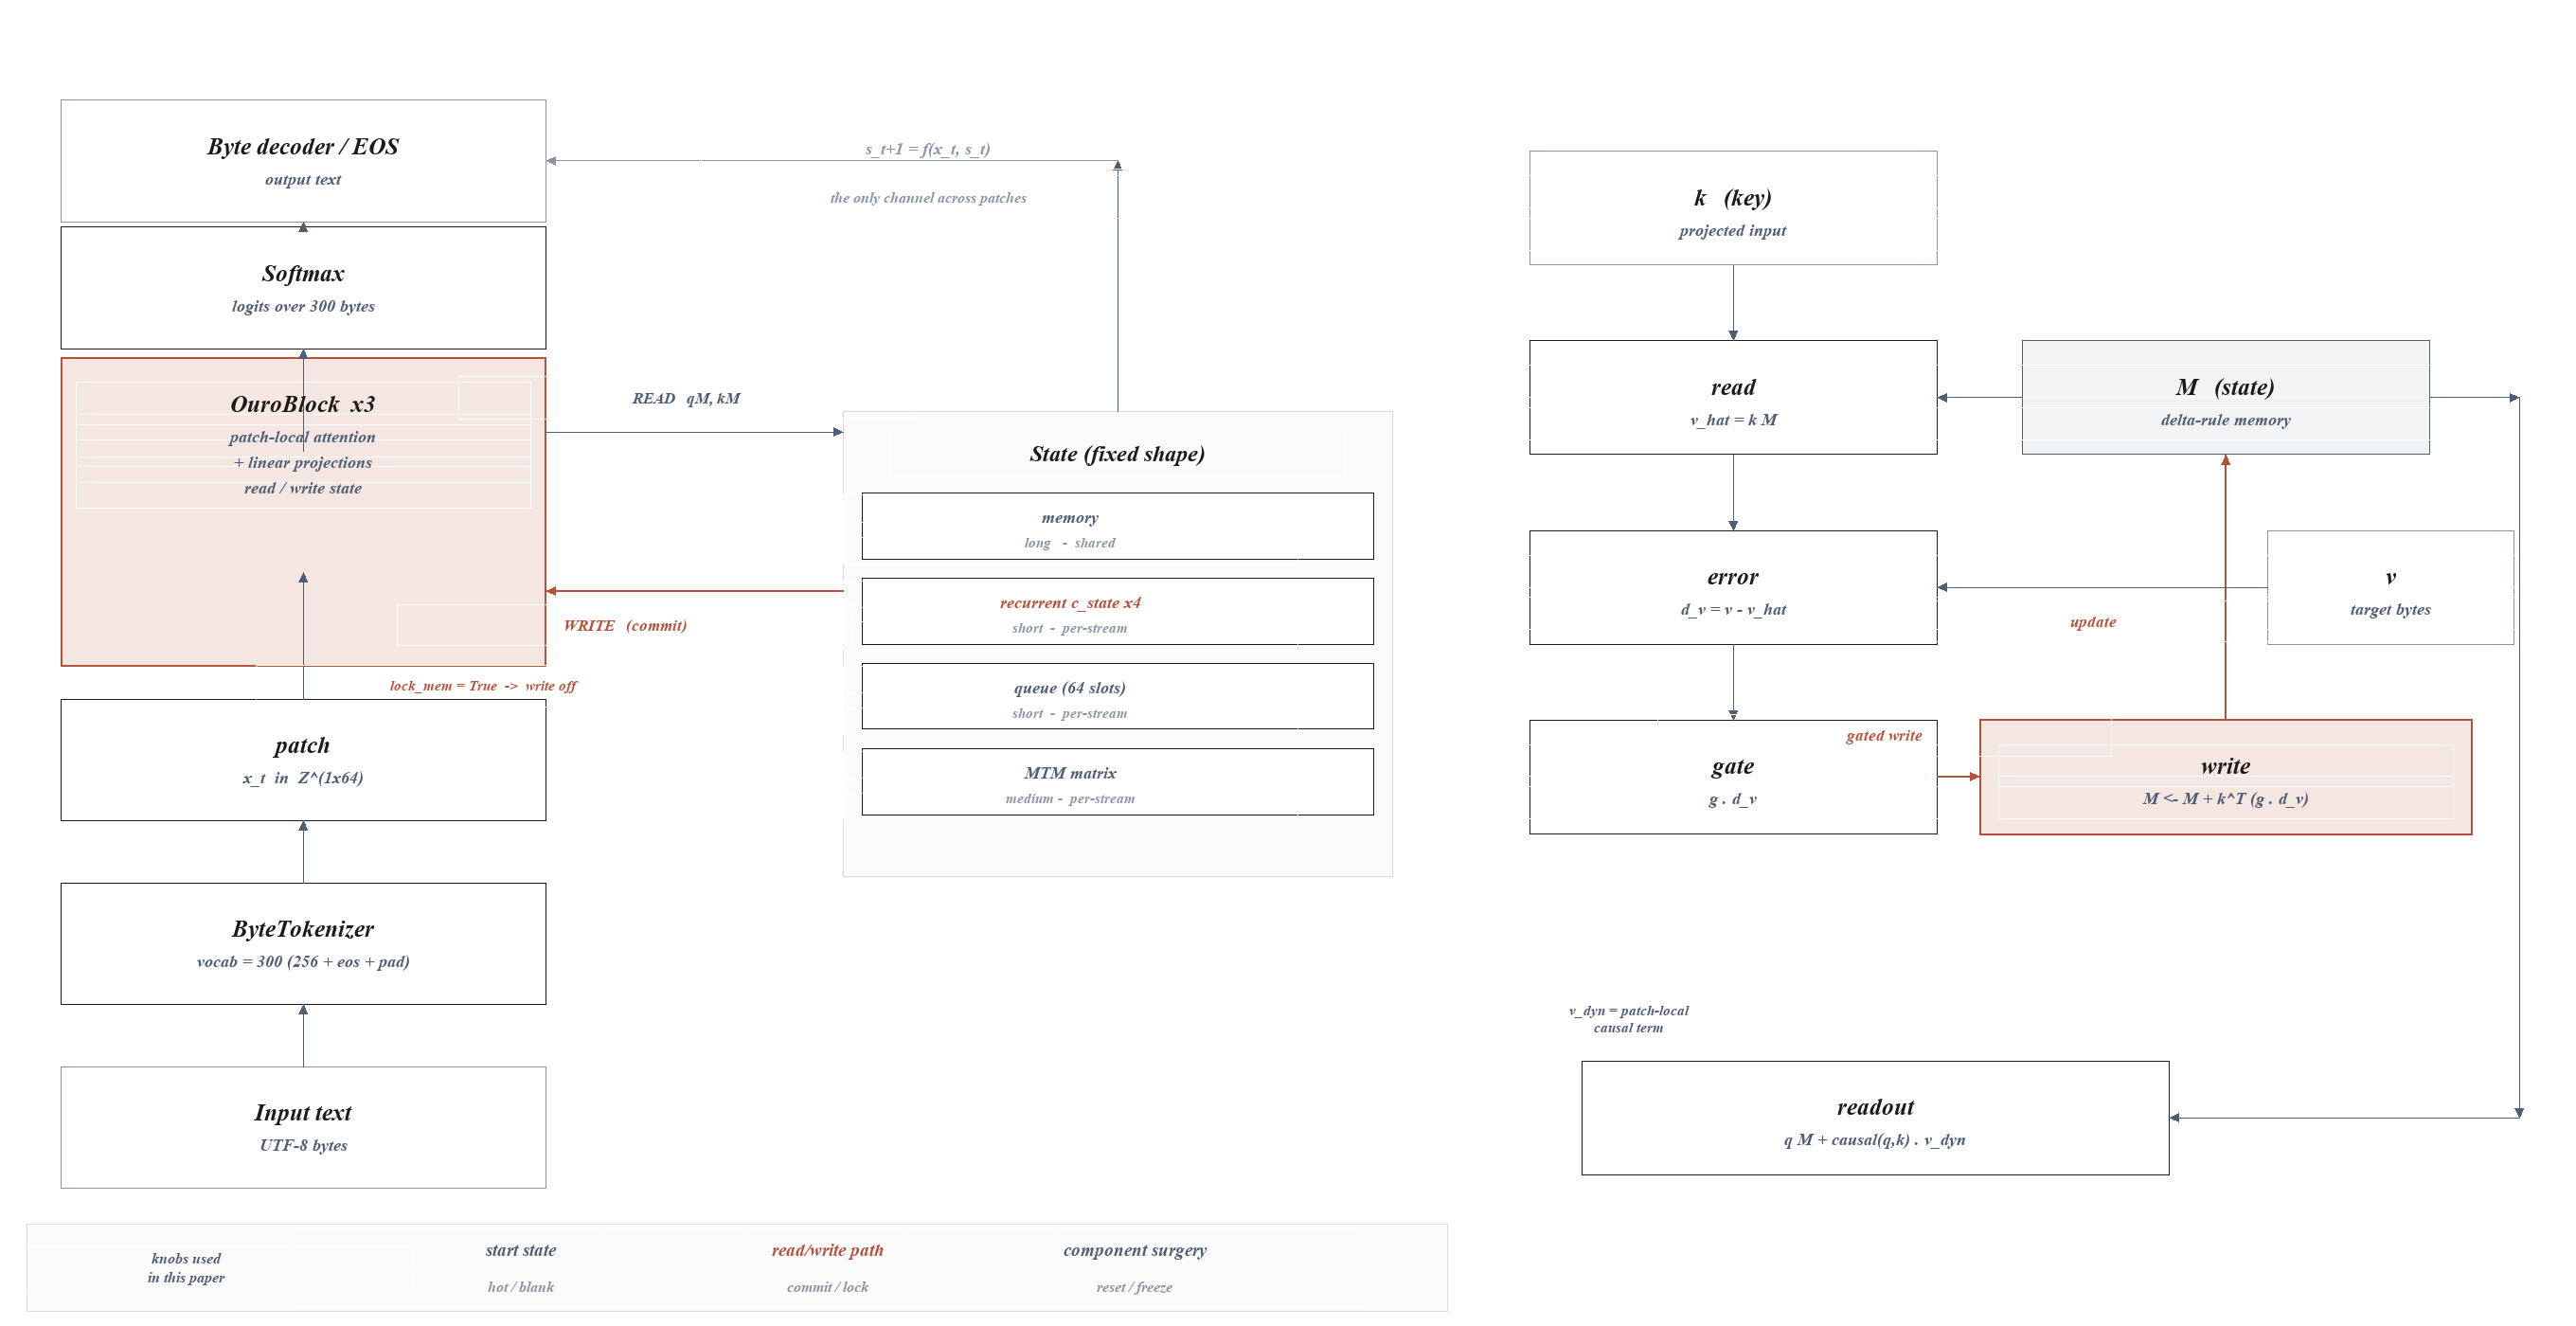
\includegraphics[width=\linewidth]{fig_arch.png}
\caption{持续状态架构与状态读写接口。左：一条跨 patch 的递归流——
输入文本经 byte 分词后在 patch 内做局部注意力混合，patch 之间的唯一信息通道是状态四件套；
右：原语 OuroCell 的读写链条（读出 $\hat v = kM$ $\to$ 误差 $\Delta v = v - \hat v$ $\to$ 门控写入
$M \leftarrow M + k^{\top}(g \cdot \Delta v)$ $\to$ 读出 $qM + \text{因果分数} \cdot v_{\mathrm{dyn}}$）。
下方给出本文实验用到的三类操纵旋钮：起点状态（热启动 / 空白）、读写路径（commit / $\mathit{lock}$）、
组件手术（重置 / 冻结）。本图由 Visio 绘制（源文件 \texttt{figs/fig\_arch.vsdx}，
用 VisioRender 渲染为 PNG；等价的矢量版本为 \texttt{figs/fig\_arch\_matplotlib.pdf}）。}
\label{fig:arch}
\end{figure}

\subsection{四件套状态及其作用域}\label{sec:model-state}

状态由四个分量构成，按时间尺度与作用域分工，见表 \ref{tab:state} 与图 \ref{fig:state-scales}。

\begin{table}[t]
\centering
\caption{状态四件套：机制、时间尺度与作用域。写入规则均为前向局部规则（无反向传播）。}
\label{tab:state}
\footnotesize
\begin{tabularx}{\linewidth}{@{}l X c X X@{}}
\toprule
分量 & 机制 & 时间尺度 & 作用域 & 写入规则 \\
\midrule
\texttt{memory} & delta 规则快权重矩阵（每层一块） & 长 & \textbf{序列级私有}（v\_0d4；v\_0d3 为跨样本共享、按流平均） & 误差驱动外积，恒等初始化 \\
\texttt{recurrent} & 块级循环状态 \texttt{c\_state}（$3+1$ 个） & 短 & 逐样本私有 & LSTM 式门控 cell \\
\texttt{queue} & 64 槽滚动队列 & 短 & 逐样本私有 & FIFO，存顶层 \texttt{c\_state} 历史 \\
\texttt{MTM} & 中期矩阵记忆 & 中 & 逐样本私有 & delta 规则，写入源为队列滑出的旧 \texttt{c\_state} \\
\bottomrule
\end{tabularx}
\end{table}

\begin{figure}[t]
\centering
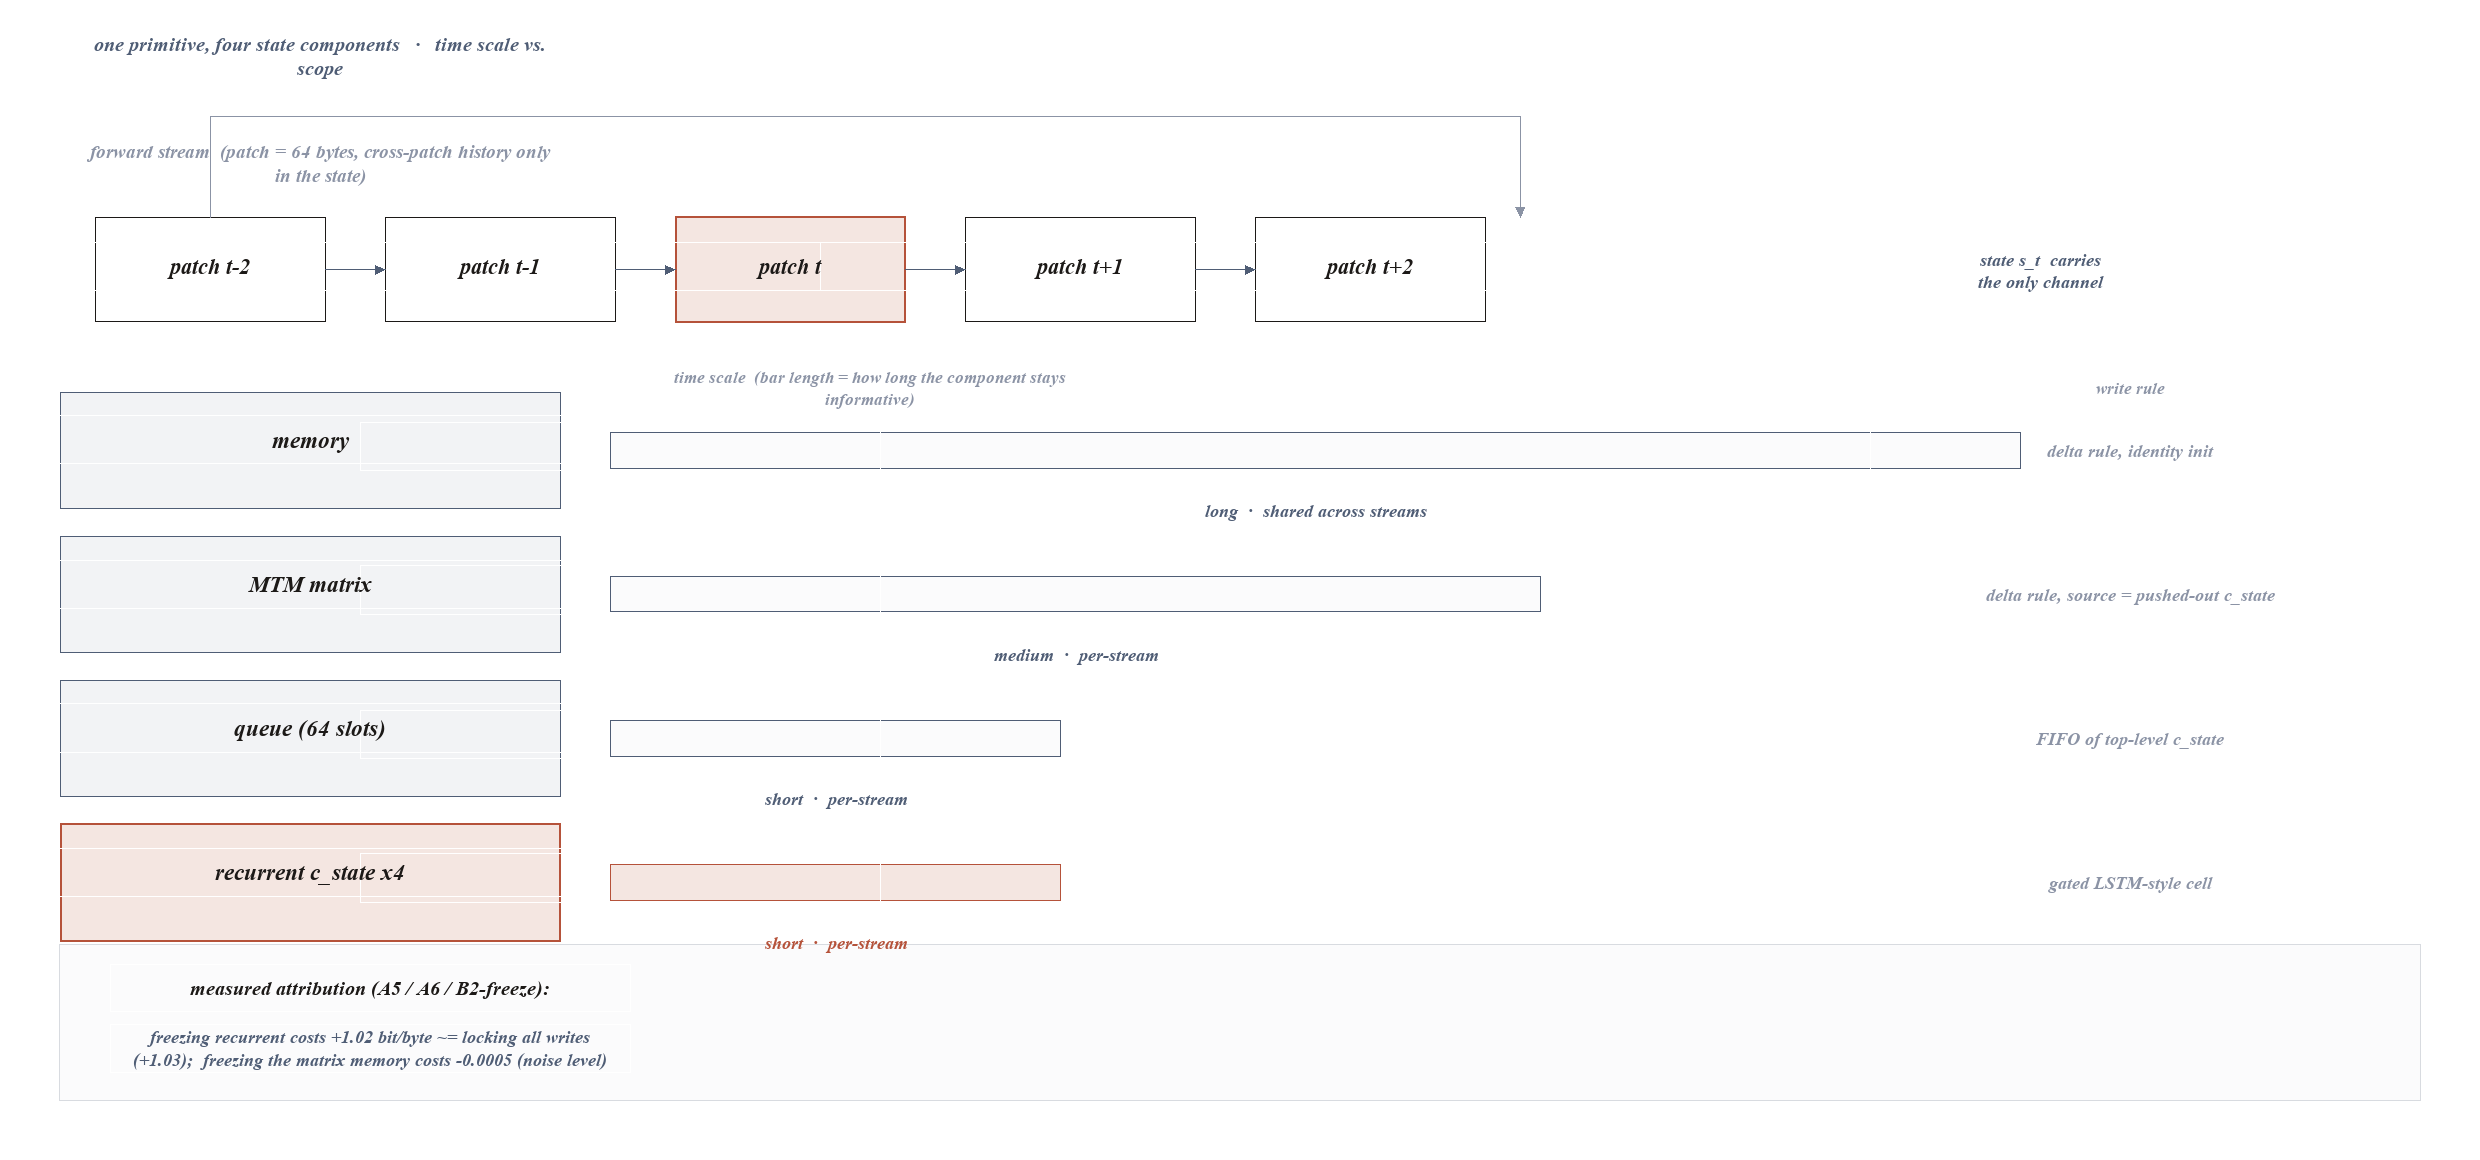
\includegraphics[width=\linewidth]{fig_state_scales.png}
\caption{四个状态分量的时间尺度与作用域（Visio 绘制，源文件 \texttt{figs/fig\_state\_scales.vsdx}）。
横条长度示意各分量「信息保持多久」的相对量级，右侧一列是写入规则；
底部给出本文实测的归属结论（A5/A6/B2-freeze 三组独立实验一致）。
注意「参数量最大的分量」并不等于「承担跨 patch 适应的分量」——这一区分由第 \ref{sec:s1} 章给出。}
\label{fig:state-scales}
\end{figure}

\textbf{作用域（按版本）。}v\_0d4 中\textbf{四个分量全部逐样本私有}——
\texttt{memory} 为每条序列独占的槽位（$[\mathrm{cap},\ldots]$，读取时按 $[:\mathrm{batch}]$ 切片），
训练提交不做跨流平均、跨卡不做同步（序列间零泄漏）。
本文检查点所属的 v\_0d3 则是「\texttt{memory} 一个共享、其余三个私有」的两族划分：
\texttt{memory} 写入后按流求均值、每 patch 一次跨卡 \texttt{all\_reduce}。
这个划分决定了「重置某个分量」实验（\S\ref{sec:s1-attr}）的语义——
在 v\_0d3 检查点上，重置 \texttt{memory} 相当于动跨样本的共享知识（本研究中等价于换回训练稳态快照），
重置其余三个只影响当前样本的上下文记忆；若换用 v\_0d4 检查点重跑，重置 \texttt{memory} 也将退化为
只影响当前样本的操作，\S\ref{sec:s1-attr} 的归因结论需要重新验证。
\textbf{本文所有实验都在 $\mathrm{batch}=1$ 上进行}，此时两版的 memory 读写逐位对应，
故推理侧结论不受该差异影响（\S\ref{sec:train}）。
\textbf{「多时间尺度」的分工叙述由实验支撑}，而不是凭结构空口断言：
本文在 \S\ref{sec:s1-attr} 用组件级重置与冻结给出分工的实测结果。

\textbf{原语。}四个分量是同一条 delta 规则在不同尺度上的实例（「一个原语、三个尺度」）：
读出 $\hat v = kM$，误差 $\Delta v = v - \hat v$，门控写入
\begin{equation}
M \leftarrow M + k^{\top}\!\left(g \cdot \Delta v\right),
\qquad g = \sigma(\cdot)\big/ \mathrm{eff\_seq\_len},
\label{eq:delta}
\end{equation}
随后读出 $qM + \text{因果分数} \cdot v_{\mathrm{dyn}}$。
式 \eqref{eq:delta} 是线性预测器的在线（岭）回归更新在秩空间中的实例，
$1/\mathrm{eff\_seq\_len}$ 缩放保证 patch 长度变化时写入量一致，门控 $g$ 使写入可以自适应减弱。

\subsection{状态的读写接口}\label{sec:model-io}

\textbf{两条前向路径：}\texttt{commit}（写入，$\mathit{lock\_mem}=\mathrm{false}$，状态正常更新）
与 \texttt{lock}（只读，$\mathit{lock\_mem}=\mathrm{true}$，状态原样直通）。
\textbf{本文所有实验的操纵旋钮都落在这两个接口上}——这是 \S\ref{sec:related-innovation} 中
「状态是微观实现、可以显式调整」的具体兑现。

\textbf{关键实现事实（受控设计的基础）：}$\mathit{lock\_mem}=\mathrm{true}$ 时四个状态分量原样直通，
因此\textbf{第一个 patch 的输出与正常前向逐位一致}——此时还没有发生任何写入；
从第二个 patch 起两者才因写入与否而分化，A2 测的就是这个分化量（\S\ref{sec:a2}）。

\textbf{推论。}状态因而是显式对象：前向返回新的状态对象而不原地修改，
所以它可以被整体读出、冻结、置换，也可以在同一份快照上并行地开出多个实验分支
（本文所有组件手术都是这个语义，见 \S\ref{sec:surgery}）。

\subsection{训练与检查点}\label{sec:train}

\textbf{状态不清零、跨批次连续（与 RNN/RWKV 的关键差别）。}
标准循环架构训练时状态从零初始化、一批读完即清零——单个状态最多跨一个样本的长度，
记忆跨不过样本边界。本文的模型\textbf{不按批次清空状态}：上一批结束时的状态直接续进下一批，
整条训练流是一条全局连续的流，状态的跨距不受样本长度限制。
batch 维被实现为若干条并行的永续数据流，\texttt{recurrent}/\texttt{queue}/\texttt{MTM} 逐流私有；
\texttt{memory} 在 v\_0d4 中同样逐流私有（每条流独占一个槽位，提交无跨流平均、跨卡无同步），
而本文检查点所属的 v\_0d3 为跨流共享（写入后按流平均，每 patch 一次跨卡 \texttt{all\_reduce}），
\texttt{chunk\_size}=192 条流。流数与 \texttt{bptt} 按版本配置：v\_0d3 为 $192$/$4$，
v\_0d4 的 MEDIUM 档改为 $1$/$16$。这正是「固定状态持续携带跨上下文信息」（S1）在训练侧成立的前提。

\textbf{记忆精度与门控初值（v\_0d4）。}记忆全程以 fp32 驻留（配置项 \texttt{mem\_dtype}，
可切 bf16 换显存，代价是小量级更新在 $|\mathrm{mem}|\!\sim\!1$ 处被舍入吸收）；
写入门控偏置初始化为 $-\ln 63\approx-4.14$，即 $\sigma(b)=1/64$，
使写入时间常数对齐 $64\times64=4096$ token 的队列视界（v\_0d3 为硬编码 $-6.0$）。

\textbf{优化与截断。}AdamW $+$ cosine 调度 $+$ 梯度裁剪 $1.0$，bf16 混合精度，
梯度窗口 \texttt{bptt}=4 个 patch（$4\times64=256$ token；本文检查点的 v\_0d3 配置，
v\_0d4 MEDIUM 档为 16 patch $=1024$ token）。
\textbf{截断窗口之外的长程信用只能经前向 delta 规则写入传递}——这是连到「持续学习」主张的关键设计点：
模型学到的不是「如何回传梯度到远处」，而是「如何在前向里把远处写进状态」。

\textbf{检查点与热启动。}训练收敛后状态达到稳态，检查点里保存的状态快照就作为评测的
\textbf{热启动}起点；若存档没有保存状态，则回退按空白处理。
存档格式随版本变化：v\_0d3 把共享 memory 存为顶层 \texttt{global\_memory} 字段（rank0 一份），
v\_0d4 把序列级 memory 放进各 rank 的 \texttt{runtime\_states}（rank 私有、全量落盘，
恢复时缺 memory 直接报错）——\textbf{两版存档互不兼容}。
本文使用 step $144{,}000/705{,}600$（约 20\% 训练进度）的中型检查点
\texttt{gridman\_medium\_v\_0d3\_pretrain}，取 batch$=1$ 切片的状态，
每次实验先克隆再跑——\textbf{状态跑一次就变}，不可复用同一对象，否则实验之间互相污染。
本文所有数字都建立在这个单一检查点上，因此\textbf{只做条件间比较}，绝对数值不可与外部模型对照（\S\ref{sec:limits}）。

\section{评测协议}\label{sec:protocol}

本节定义贯穿全文的评测协议。所有实验脚本共享同一套脚手架：模型单例 + 热启动状态 + teacher-forced
流式评测 + 文本源切分 + 组件手术工具。

\subsection{数据与 held-out 切分}\label{sec:data}

\textbf{语料。}预训练语料为 \texttt{pretrain.jsonl}（约 9.5\,GB，每行 \texttt{\{"text": ...\}}），
微调语料为 \texttt{sft.jsonl}（约 14\,GB，每行多轮对话）。训练按流（stream）组织：
本文检查点（v\_0d3）为 \texttt{chunk\_size}=192 条并行流，每条流对应文件的一段连续 chunk（约 49.4\,MB）。

\textbf{零污染 held-out。}训练在 step $144{,}000$ 时，每条流已消费 $144{,}000\times64\ \mathrm{B}=9.2$\,MB
（这是从训练步数与 patch 长度推算的上界）。因此本文从每条流 chunk 内\textbf{偏移 $\ge20$\,MB 处}取行，
再按 seed 洗牌拼成评测文本——取行位置远超已消费区，属同分布零污染。
\textbf{跨域档}取 \texttt{sft.jsonl} 尾部（深度按 seed 随机化）；
\textbf{消费区档}（成员推断用）取流 0 chunk 内 $[0.5,7]$\,MB 的随机偏移，
即训练确实见过的文本。$\mathrm{n}$-gram 重叠率报告的精确统计 \pending{待补：4-gram 重叠率明细见附录 \ref{app:decontam}}。

\textbf{合成档。}可打印 ASCII（字节 $\in[33,122]$，刻意 OOD）与词表内高频词对（分布内）两类，
用于前向学习与遗忘类实验（附录 \ref{app:c1}、\ref{app:g}）。

\subsection{主指标：teacher-forced bits/byte}\label{sec:metric}

\textbf{前向协议完全镜像训练前向：}patch 大小 $64$、相邻窗口重叠 1 字节
（输入 \texttt{ids[64k:64k+64]}，目标 \texttt{ids[64k+1:64k+65]}），
$\mathrm{model.eval}()$ + bf16 autocast + \texttt{inference\_mode}，不做生成式采样。
指标为 teacher-forced 交叉熵，以 \textbf{bits/byte}（$=\mathrm{nats}/\ln 2$）报告；
机会线为 $\log_2 300 \approx 8.23\ \mathrm{bit/byte}$（对 300 个字节均匀瞎猜）。

\textbf{状态流必须逐 patch 推进。}评测不能跳过任何 patch 的前向——跳过会冻结状态推进，
测出来的就不是同一条流（本文实验中都只跳过「计分」，不跳过「前向」）。

\textbf{口径说明（两处容易混淆的细节）。}
（i）当所有计分 patch 长度相同时，「每 patch 均值的均值」与「每 token 均值」严格相等，
因此 bits/byte 与逐 token 均值可以直接互换；本文实验脚本中两种实现都出现过，
所有报告数字都在等长 patch 窗口上取得，故不受该差异影响。
（ii）$\mathrm{n}$-gram 复现类指标（\S\ref{sec:b2}）的「距离」以字节计，在本模型中字节即 token。

\subsection{起点状态与实验条件声明}\label{sec:cond}

按「每次评测显式声明 \{\,起点状态,\, $\mathit{lock}$ 与否,\, 重置点\,\}」的约定，
本文所有结果表都标注这三个条件。起点状态三种来源：
\textbf{热启动}（训练稳态快照）、\textbf{空白}（恒等 memory $+$ 零 recurrent/queue/MTM）、
\textbf{热启动 $+$ 插件}（如仅回滚 \texttt{memory} 或仅清零 \texttt{recurrent}，见 \S\ref{sec:surgery}）。

\textbf{关于空白态的适用性。}空白起步使 delta 规则写读链路偏离训练操作点，
它在损失上表现为结构性失效（\S\ref{sec:a1}），因此本文\textbf{不以空白作为主表基线}，
而以热启动为基线、以「热启动 $-$ 空白」的差作为「状态贡献」的度量，
并把空白的绝对水平仅用作参照。出于同一原因，凡涉及「模型记住了训练语料吗」的问题
（\S\ref{sec:dline}），必须\textbf{双报}两种起点。

\subsection{统计口径}\label{sec:stats}

\textbf{（i）文本真随机化。}同一实验的多个 seed 必须改变\textbf{取文本的偏移}，
否则多个「seed」实际是同一段文本，会给出假窄的置信区间（本文脚手架在早期版本犯过该错并已修正）。
\textbf{（ii）成对报告。}凡是同一文本上的两条件对照（如 write vs $\mathit{lock}$），
先算每个 seed 的差值再取均值，而非分别取均值后相减——前者剔除了文本难度差异。
\textbf{（iii）置信区间。}报告 $1.96\times\mathrm{std}/\sqrt{n}$ 的 95\% 区间；$n\le2$ 时区间仅作参考。
\textbf{（iv）显存卫生。}连续执行多个短评测任务时逐次清空 CUDA 缓存分配器（否则会累积到 OOM，实测 25\,GB）。
\textbf{（v）确认性与探索性的区分。}第 \ref{sec:s1} 章的状态消融（A1--A6）与 B2 的主结论属于\textbf{确认性}实验：
成立条件在跑之前就写明（\S\ref{sec:problem}），实现缺陷订正后重跑仍成立。
而\textbf{自然重复的距离分桶}（\S\ref{sec:b2} 的表 \ref{tab:b2}）是\textbf{探索性/事后分组}：
桶边界由我们选定，不同距离上重复的是不同的 $\mathrm{n}$-gram 群体，因此该表用于描述形状而非做显著性检验。
附录 \ref{app:dline}--\ref{app:g} 的 D/E/G 三线（状态知识性质、稳定性、前向学习）
是在主结论之后追加的探索，用于解释机制，不承担主 claim。

\textbf{（vi）数字溯源。}本文每张表的每个数字都可追到实验包里的一个结果文件：
附录表 \ref{tab:config} 给出「脚本 $\leftrightarrow$ 实验」的对应关系，
结果文件命名统一为 \texttt{stage*\_results.json}（A1 为 \texttt{a1\_*\_per\_patch.json}）；
改口径即重跑、重跑即换文件，不做手工誊抄。表中未取得的数据一律标 \pending{}，不以估计值填充。

\subsection{状态手术：本文的操纵旋钮}\label{sec:surgery}

由于状态是显式、不可变的对象（\S\ref{sec:model-io}），本文可以在任意 patch 边界对状态做手术。
协议共用到五类操作（图 \ref{fig:protocol}），全部实现为「在某个 patch 前/后把状态替换为新对象」：

\begin{table}[t]
\centering
\caption{状态手术工具及其语义。所有操作都只改状态、不改权重。}
\label{tab:surgery}
\footnotesize
\begin{tabularx}{\linewidth}{@{}l X l@{}}
\toprule
操作 & 语义 & 用于 \\
\midrule
\texttt{lock\_mem} & 跨 patch 的持久写入关闭（patch 内 $v_{\mathrm{dyn}}$/因果分数仍在工作） & A2、B2、G2 \\
\texttt{reload\_hot\_memory} & 仅 \texttt{memory} 回训练稳态快照 & A5 \\
\texttt{zero\_recurrent} & 仅 \texttt{recurrent} 清零 & A5、C 线 \\
\texttt{blank\_queue\_mtm} & \texttt{queue} 清零 $+$ \texttt{MTM} 回恒等 & A5、C 线 \\
\textbf{freeze}$_{\text{子集}}$ & 每个 patch 前向后把指定分量子集恢复为前值（该分量跨 patch 不更新，patch 内照常更新） & A6、B2-freeze \\
\bottomrule
\end{tabularx}
\end{table}

\begin{figure}[H]
\centering
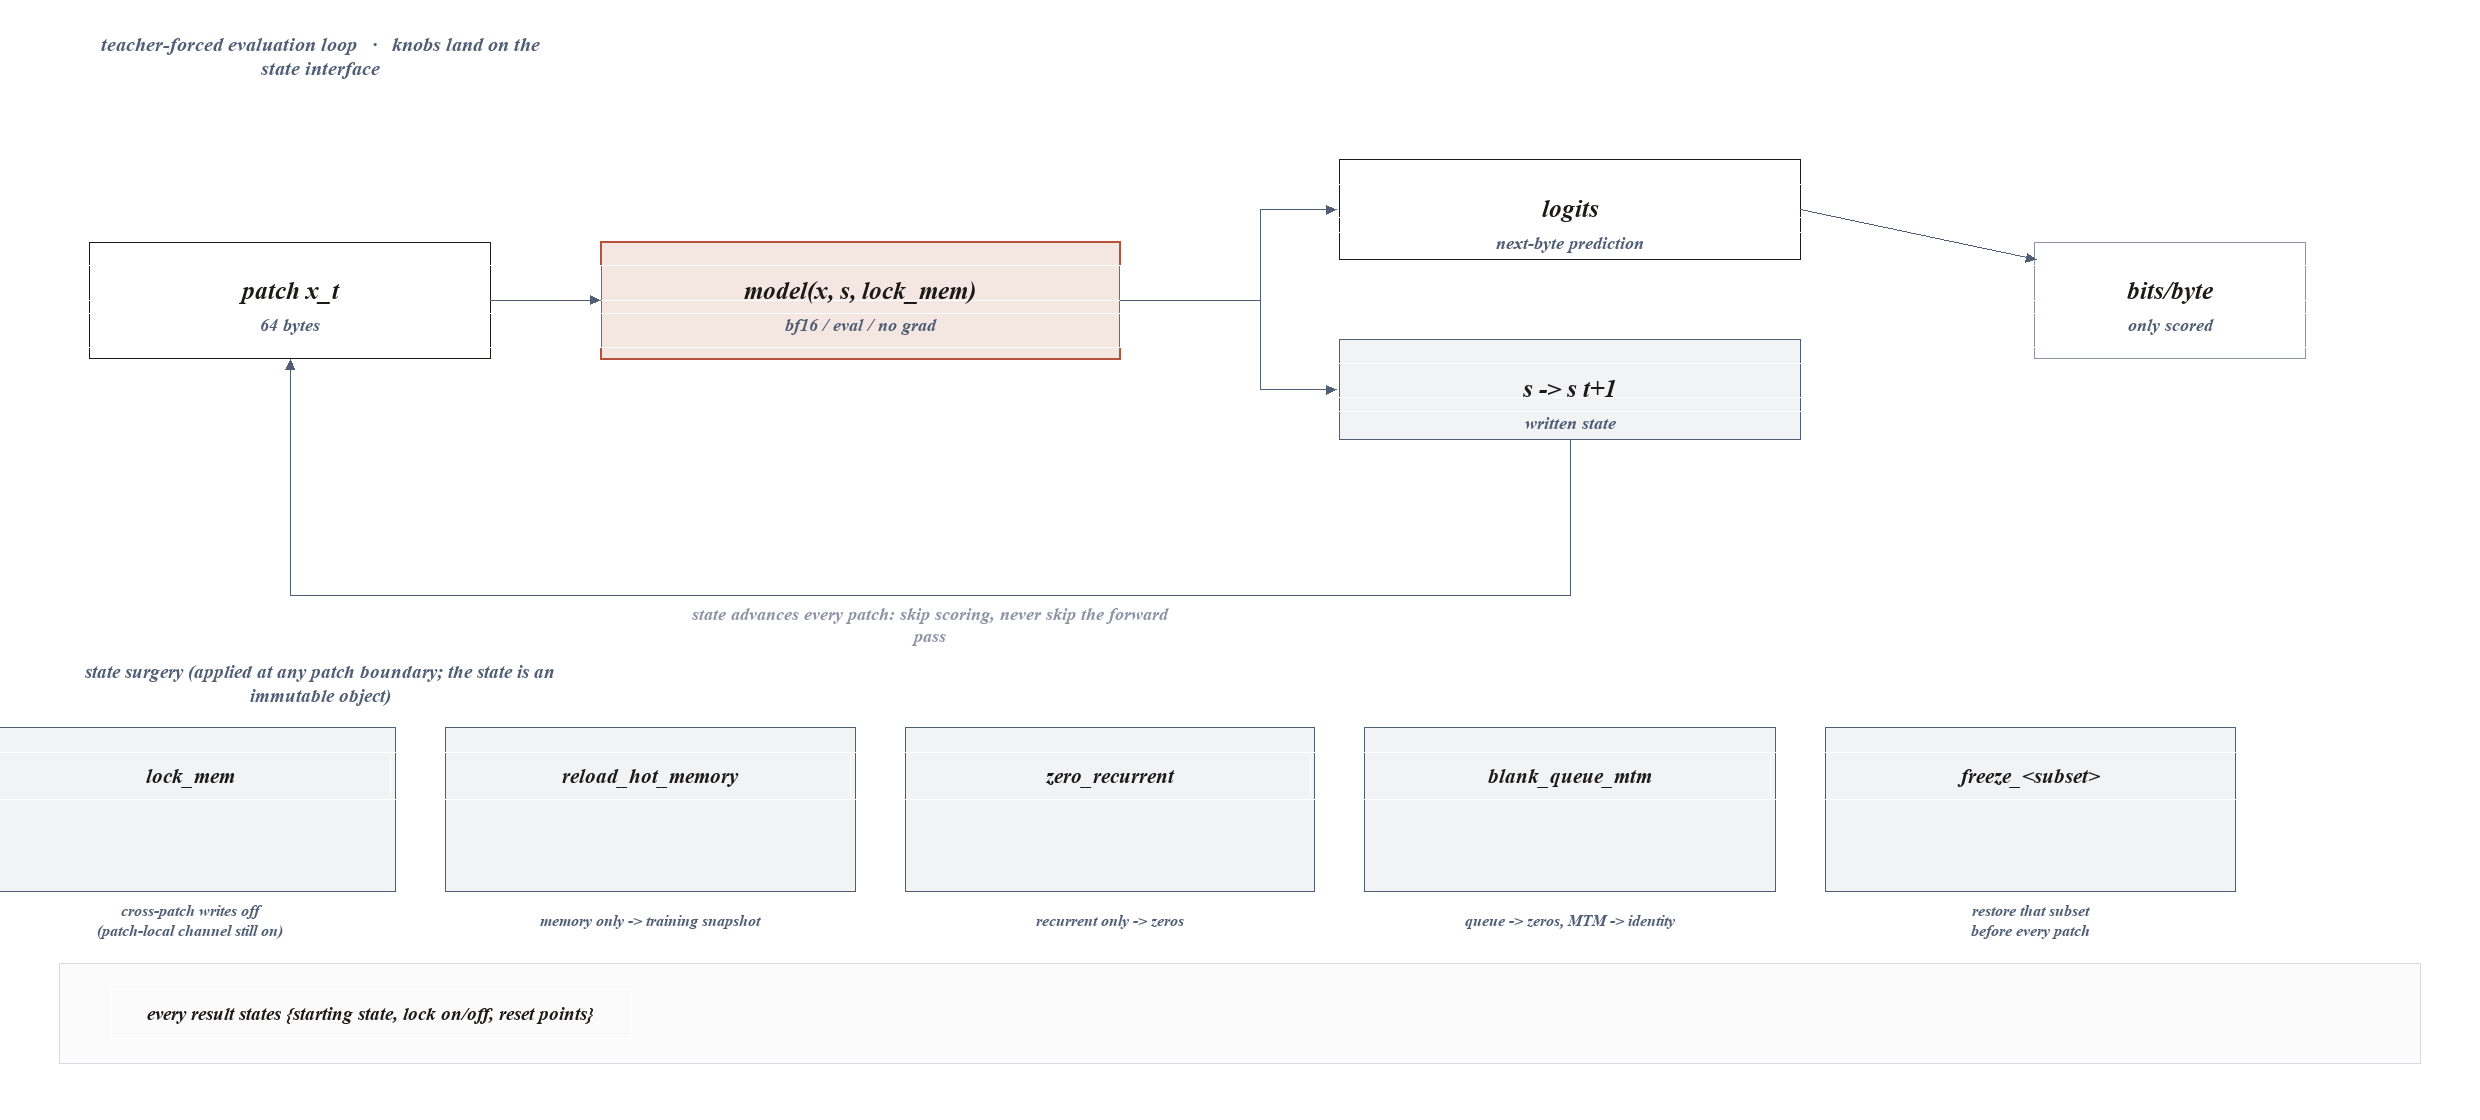
\includegraphics[width=\linewidth]{fig_protocol.png}
\caption{teacher-forced 评测回路与状态手术（Visio 绘制，源文件 \texttt{figs/fig\_protocol.vsdx}）。
每个 patch 都必须前向（跳过会冻结状态推进，只允许跳过计分）；五类手术都在 patch 边界上把状态换成新对象，
因此互不干扰的实验分支可以在同一份快照上并行开出。}
\label{fig:protocol}
\end{figure}

\textbf{$\mathit{lock}$ 与 freeze 的区别必须写清。}$\mathit{lock\_mem}$ 关闭的是\textbf{跨 patch 的持久写入}，
patch 内的动态通道仍然工作；freeze 是逐分量版本——它冻结的是某一个分量在跨 patch 尺度上的更新，
其余分量照常参与。两者互为「全局/组件」两种粒度的同一干预，
这正是 \S\ref{sec:s1-attr} 能把「写入收益」拆到组件上的原因。

\textbf{勘误与协议纪律。}本文在成稿前对实验包做了逐脚本审读，发现并订正了三处口径问题，
其中两处影响数字、一处影响结论：$\mathrm{n}$-gram 分桶的一处实现缺陷（导致「长程零衰减」的错误结论，
已修复重跑，见 \S\ref{sec:b2}）；A1 的计分窗口未对齐（已改为所有条件共用同一窗口，见 \S\ref{sec:a1}）；
受控遗忘曲线的答案位置整体偏移 66 字节（实验作废，说明见附录 \ref{app:c1}）。
这三处订正都已落到脚本里，并配了一个模型无关的位置自检脚本作为回归测试。

\section{实验一：起点状态（子主张 S1）}\label{sec:s1}

本章逐组给出起点状态的消融结果（总览见图 \ref{fig:ablation}），回答 S1 的两个成立条件：
\textbf{热启动是否显著优于空白}（\S\ref{sec:a1}）与\textbf{写入是否显著优于 $\mathit{lock}$}（\S\ref{sec:a2}），
再用跨文档边界（\S\ref{sec:a3}）与组件级归因（\S\ref{sec:s1-attr}）回答「信息由谁承载」。

\begin{figure}[H]
\centering
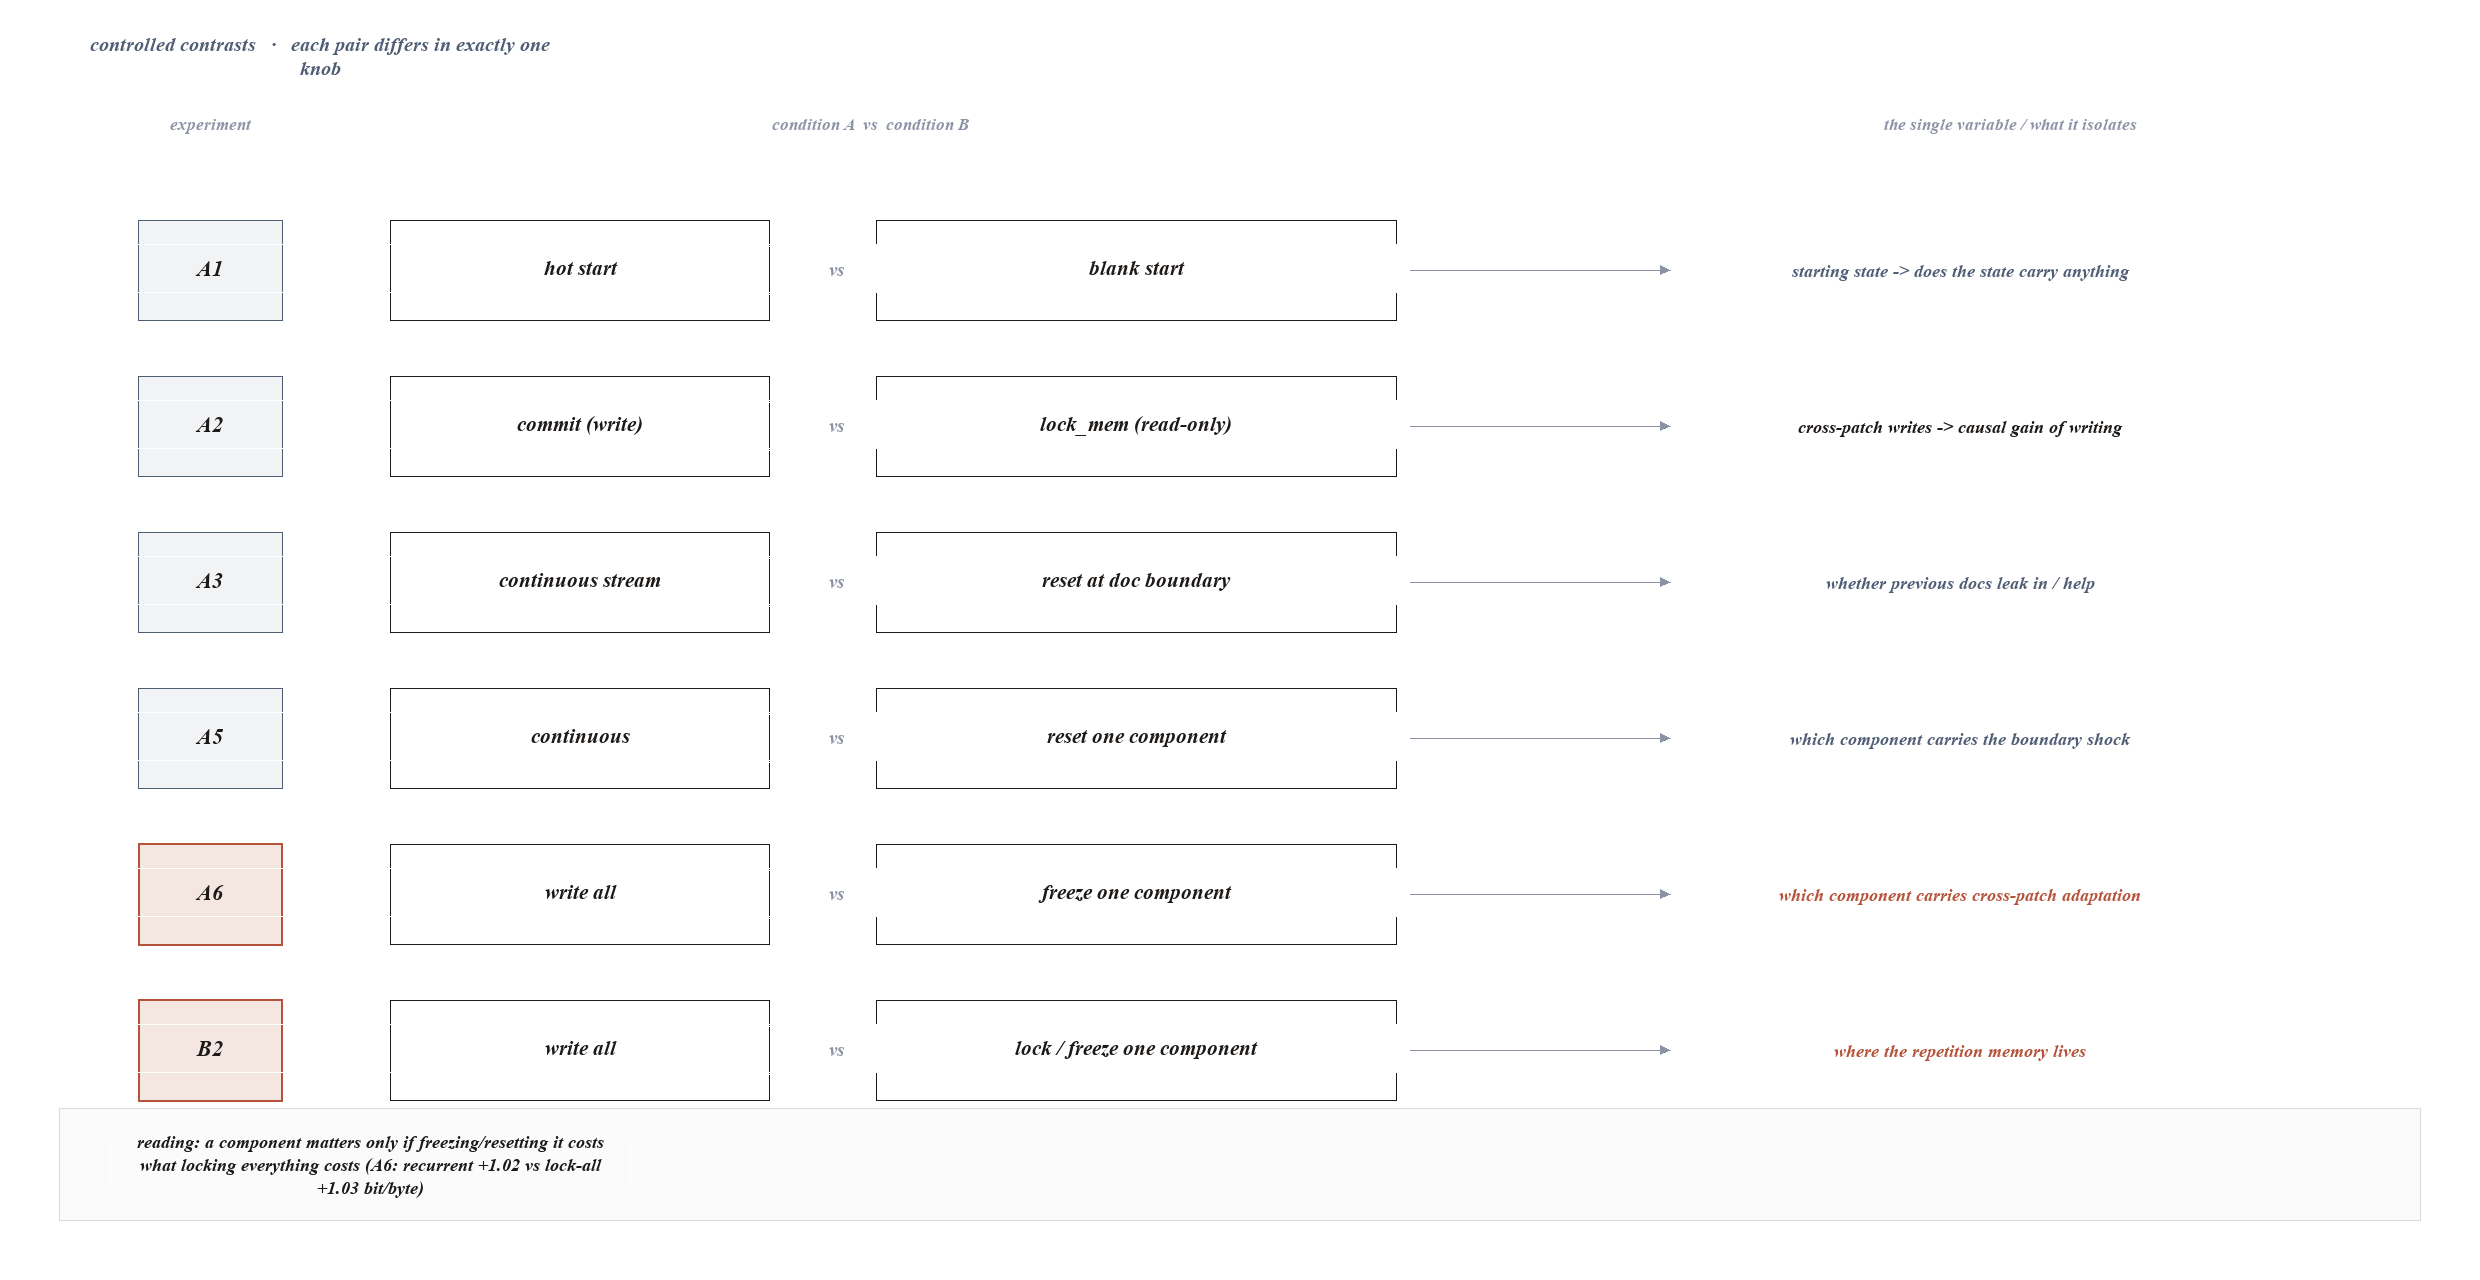
\includegraphics[width=\linewidth]{fig_ablation_matrix.png}
\caption{受控对照一览（Visio 绘制，源文件 \texttt{figs/fig\_ablation\_matrix.vsdx}）。
每一对条件只差一个旋钮；右侧一列写出该对照隔离出的变量。
阅读方式写在图底：一个分量只有在「冻结/重置它的代价等于冻结全部写入的代价」时，才算真正承载了这门功能。}
\label{fig:ablation}
\end{figure}

\subsection{热启动 vs 空白起步（A1）}\label{sec:a1}

\textbf{设计。}同一份文本、同一前向协议，唯一变量是初始状态：
热启动（\texttt{load\_model\_checkpoint} 取训练稳态快照）对空白
（\texttt{init\_inference\_state}：恒等 memory $+$ 零 recurrent/queue/MTM）。
\textbf{计分窗口对齐}：三个「空白 $+$ 预热 $W$ token」档（$W\in\{0,256,1024\}$）在实现上只是
「从第 $W/64$ 个 patch 起计分」——每个 patch 都会被前向，所以三档的状态轨迹完全相同。
既然状态轨迹相同，三档就必须在\textbf{同一个计分窗口}上比较，否则「预热」只是个伪变量。
本文按此对齐：所有条件一律从第 16 个 patch 起计分。

\textbf{结果（表 \ref{tab:a1}、图 \ref{fig:a1}）。}对齐窗口（48 个 patch $=$ 3\,KB，文本取自 sft 尾部 4097 字节）：
热启动 $1.588\bits$，空白 $5.319\bits$，差距 $\mathbf{3.731\bits}$。
三个空白档在对齐窗口上的数值\textbf{逐位相同}（最大差 $0.000\mathrm{e}{+}0$）——这直接印证了
「预热档是伪变量」。窗口内\textbf{无追平趋势}（图 \ref{fig:a1} 右：$blank-hot$ 全程在 $1.1$--$4.6\ \nats$ 之间波动，无下行）。

若不做窗口对齐（即照早期报告的写法），三档分别是 $5.668/5.544/5.319\bits$，
其中「$0.35$ bits 的挽回」全部来自把最差的头几个 patch 排除在计分之外，
而不是模型写得慢——这一点必须在论文里写清，否则会误读成「空白态可以通过预热追上」。

% A1：热启动 vs 空白起步（对齐计分窗口）
\begin{table}[t]
\centering
\caption{A1 热启动 vs 空白起步。文本为 \texttt{sft.jsonl} 尾部 4097 字节（跨域、零污染），
所有条件记分窗口相同（第 16--63 个 patch，共 48 个 patch $=$ 3\,KB）。
「预热」档在对齐窗口上数值逐位相同（最大差 $0.000\mathrm{e}{+}0$），故不是有效变量；
最后一行给出未对齐窗口时的数值，两者相差的 $0.35\bits$ 纯属窗口效应。}
\label{tab:a1}
\small
\begin{tabular}{@{}lccc@{}}
\toprule
条件 & 起点状态 & 计分窗口 & bits/byte \\
\midrule
热启动（hot） & 训练稳态快照 & 48 patch（对齐） & $\mathbf{1.588}$ \\
空白（blank） & 恒等 memory $+$ 零其余 & 48 patch（对齐） & $5.319$ \\
空白 $+$ 预热 256 & 同上（同一轨迹） & 48 patch（对齐） & $5.319$ \\
空白 $+$ 预热 1024 & 同上（同一轨迹） & 48 patch（对齐） & $5.319$ \\
\midrule
\multicolumn{2}{@{}l}{热启动 $-$ 空白（对齐窗口）} & 48 patch & $\mathbf{+3.731}$ \\
\midrule
热启动（未对齐） & 训练稳态快照 & 64 patch & $1.623$ \\
空白 $+$ 预热 0（未对齐） & 恒等 memory $+$ 零其余 & 64 patch & $5.668$ \\
空白 $+$ 预热 256（未对齐） & 同上 & 60 patch & $5.544$ \\
\bottomrule
\end{tabular}
\end{table}


\begin{figure}[t]
\centering
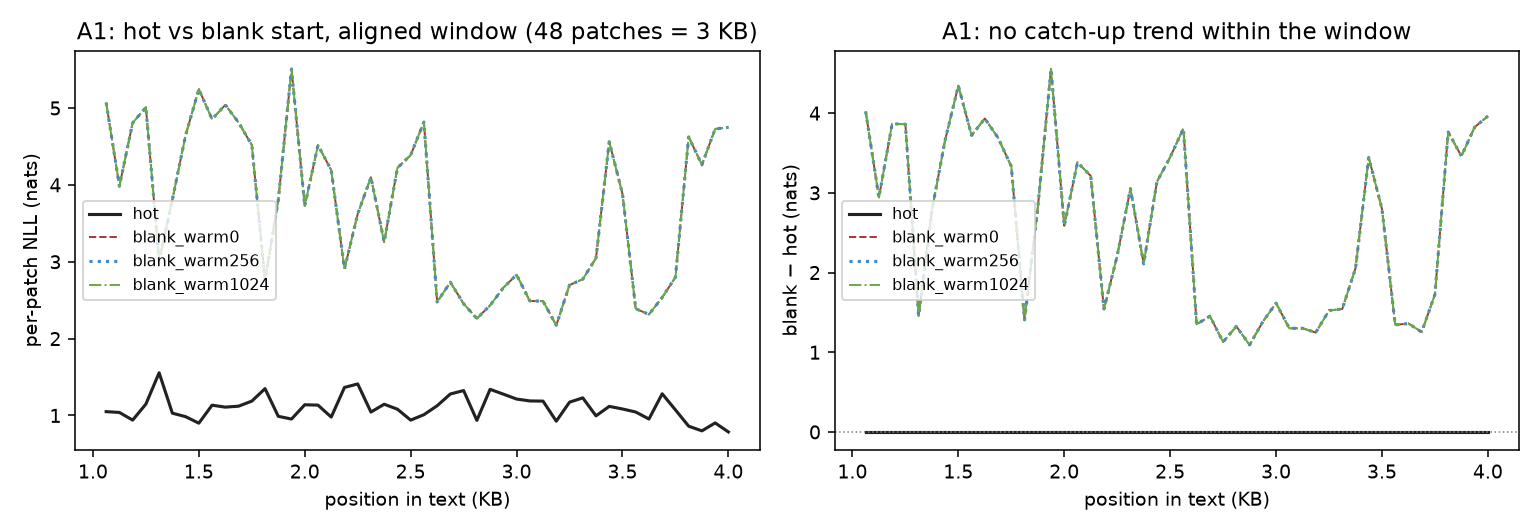
\includegraphics[width=\linewidth]{fig_a1_hot_vs_blank.png}
\caption{A1：热启动 vs 空白起步（同一计分窗口，48 个 patch $=$ 3\,KB）。
左：逐 patch NLL；三条空白曲线\textbf{完全重合}（预热档同一计算），热启动全程低 $1$--$4\ \nats$。
右：$blank-hot$ 的差值曲线，窗口内无收敛趋势。}
\label{fig:a1}
\end{figure}

\textbf{判定。}S1 的第一条成立：热启动显著优于空白，且差距不是「写入速度」能解释的
（对齐窗口内空白没有变小趋势）。
\textbf{推论与限定}：空白态的差是结构性的——恒等/零状态使 delta 规则的读写链路偏离训练操作点，
前向通道在空白态下并未进入正常工作区。因此空白\textbf{不能}作为「无记忆」的干净对照，
只能作为「状态贡献」的上界演示；热启动记忆的成分分解（通用先验 / 同分布偏向 / 逐样本痕迹）
见 \S\ref{sec:dline}。

\subsection{写入的因果贡献：$\mathit{lock}$ 对照（A2）}\label{sec:a2}

\textbf{设计。}同一份同分布 held-out（16\,KB，seed $\in\{0,1,2\}$ 三份不同文本），
两个条件：\texttt{write}（正常 commit）与 \texttt{lock}（$\mathit{lock\_mem}=\mathrm{true}$，
跨 patch 持久写入关闭）。由于 $\mathit{lock}$ 不改变首个 patch 的输出（\S\ref{sec:model-io}），
两条件在前 64 字节逐位一致，差异只来自「从第二个 patch 起，这段上下文是否被写进状态」。
指标为 bits/byte，并按 seed 成对求差（\S\ref{sec:stats}）。

\textbf{结果（表 \ref{tab:a2}、图 \ref{fig:a2}）。}
$\mathrm{write}=1.581\pm0.493$、$\mathrm{lock}=2.580\pm0.399\bits$，
\textbf{成对差值 $=+0.999\pm0.095\bits$}（三份文本分别为 $0.978/1.091/0.927$）。
逐 patch 看，差值\textbf{随后段增长}：前 32 个 patch $+0.585\nats$、后 32 个 patch $+0.771\nats$——
写入的收益是\textbf{累积}的。

% A2：写入 vs 只读（lock）
\begin{table}[t]
\centering
\caption{A2 写入 vs 只读（$\mathit{lock\_mem}$）。同分布零污染 held-out 16\,KB，
三个 seed 为三份不同文本。主报\textbf{成对差值}（先算每份文本的差再平均），
它剔除了文本难度差异；末两行为 seed 0 的逐 patch 差值演化，显示写入收益随上下文累积。}
\label{tab:a2}
\small
\begin{tabular}{@{}lccc@{}}
\toprule
seed（文本） & write (bits/byte) & lock (bits/byte) & 差值（lock $-$ write） \\
\midrule
0 & $1.661$ & $2.639$ & $+0.978$ \\
1 & $1.111$ & $2.202$ & $+1.091$ \\
2 & $1.971$ & $2.899$ & $+0.927$ \\
\midrule
均值 $\pm$ 95\% CI & $1.581\pm0.493$ & $2.580\pm0.399$ & $\mathbf{+0.999\pm0.095}$ \\
\midrule
\multicolumn{4}{@{}l}{seed 0 逐 patch 差值（nats）：前 32 patch $+0.585$；后 32 patch $+0.771$} \\
\bottomrule
\end{tabular}
\end{table}


\begin{figure}[t]
\centering
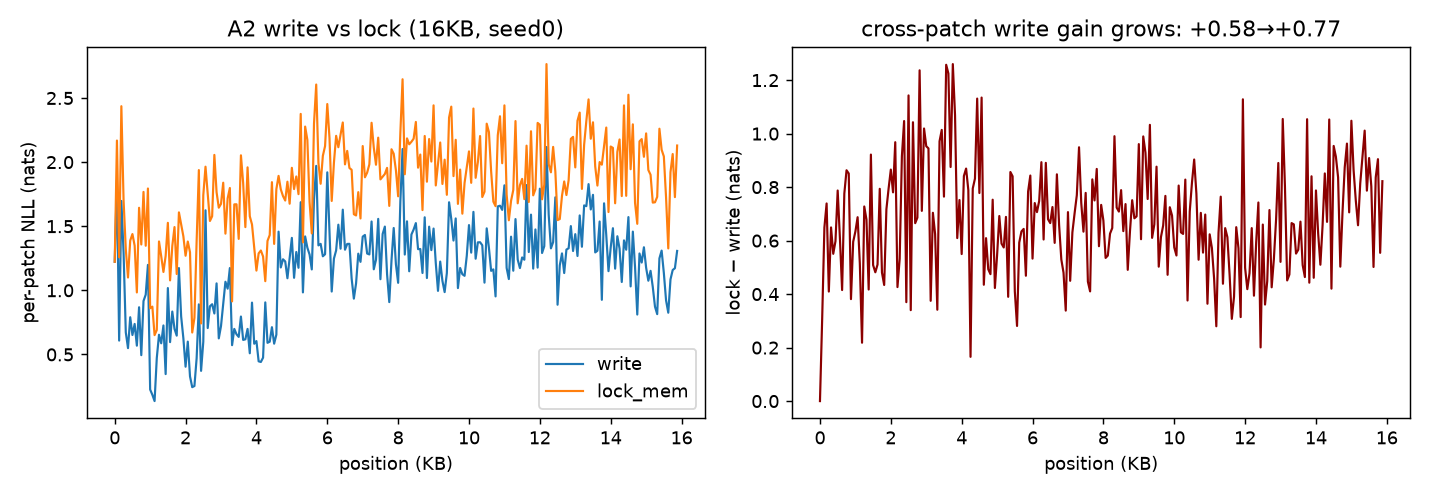
\includegraphics[width=\linewidth]{fig_a2_write_vs_lock.png}
\caption{A2：写入 vs 只读（16\,KB，seed 0）。左：逐 patch NLL；右：$\mathit{lock}-\mathrm{write}$ 的差值，
随上下文增长而增大（前段 $+0.58\to$ 后段 $+0.77$ nats），即跨 patch 写入的收益在累积。}
\label{fig:a2}
\end{figure}

\textbf{判定。}S1 的第二条成立：跨 patch 写入对预测有稳定、可累积的正贡献。
\textbf{注意语义}：$\mathit{lock}$ 只冻结\textbf{跨 patch 的持久写入}，
patch 内的动态通道（$v_{\mathrm{dyn}}$ 与因果分数）仍在工作（表 \ref{tab:surgery}），
所以该对照隔离的是「跨 patch 写入」，不是「全部记忆效应」；
把这一收益拆到具体分量，见 \S\ref{sec:s1-attr}。

\subsection{跨文档边界的信息延续（A3）}\label{sec:a3}

\textbf{设计。}16 篇文档 $\times$ 3072\,B（共 768 个 patch、15 个边界）拼成一条流，
条件：
\textbf{continuous}（状态连续跨文档，即训练时的行为）、
\textbf{reset\_full}（每个边界把状态重置回热启动全态）、
以及重置单个分量的三个变体（在 \S\ref{sec:s1-attr} 中报告）。
指标：整体 bits/byte、边界后 2 个 patch 相对边界前基线的冲击（nats）、
以及回落到「基线 $+0.5\nats$ 以内」所需 patch 数（恢复长度）。

\textbf{结果（表 \ref{tab:a3}、图 \ref{fig:a3}）。}
连续 $1.1032$ 对全重置 $1.1281\bits$；后 14 篇（跳过前 2 篇 burn-in）的平均 NLL：
连续 $0.7711$ 对全重置 $0.7903\nats$，跨文档增益 $-\mathbf{0.0192}\nats$。
边界冲击 $+\mathbf{0.4504}\nats$，恢复长度\textbf{中位数 1 个 patch、最大 2 个 patch}（$n=15$ 个边界）。

% A3 + A5：文档边界与单组件重置
\begin{table}[t]
\centering
\caption{A3 跨文档边界（16 篇文档 $\times$ 3072\,B $=$ 768 patch、15 个边界）与 A5 单组件重置。
冲击 $=$ 边界后 2 个 patch 的平均 NLL 相对边界前 8 个 patch 基线的增量；
恢复长度 $=$ 回落到「基线 $+0.5$\,nats」以内所需的 patch 数。
连续条件无重置点，故不给冲击/恢复。}
\label{tab:a3}
\small
\begin{tabular}{@{}lcccc@{}}
\toprule
条件 & bits/byte & 后段 NLL (nats) & 边界冲击 (nats) & 恢复（中位 / 最大） \\
\midrule
continuous（不重置） & $1.1032$ & $0.7711$ & --- & --- \\
reset\_full（全部重置） & $1.1281$ & $0.7903$ & $+0.4504$ & $1 / 2$ \\
reset \texttt{recurrent} & $1.1241$ & $0.7875$ & $+0.3779$ & $1 / 2$ \\
reset \texttt{memory} & $1.1029$ & $0.7709$ & $+0.0246$ & $0 / 1$ \\
reset \texttt{queue}$+$\texttt{MTM} & $1.1026$ & $0.7708$ & $+0.0250$ & $0 / 1$ \\
\midrule
\multicolumn{5}{@{}l}{跨文档增益（continuous $-$ reset\_full，后 14 篇）：$-0.0192$\,nats；
\ \ \texttt{recurrent} 解释边界冲击的 $84\%$} \\
\bottomrule
\end{tabular}
\end{table}


\begin{figure}[H]
\centering
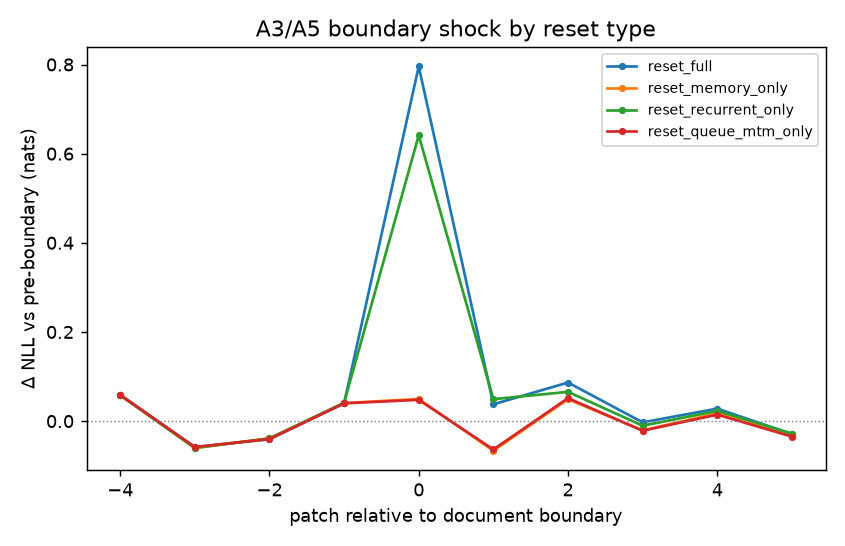
\includegraphics[width=\linewidth]{fig_a3_boundary_recovery.png}
\caption{A3/A5：以文档边界为原点对齐的平均恢复曲线（16 篇文档、15 个边界）。
全部重置的冲击明显；单组件重置的曲线给出归因——\texttt{recurrent} 的曲线几乎复现全重置冲击，
\texttt{memory} 与 \texttt{queue+MTM} 的重置几乎免费。}
\label{fig:a3}
\end{figure}

\textbf{判定。}跨文档的信息延续\textbf{真实但量级小}（$\sim0.02\nats$）；
而边界冲击虽然尖锐（$+0.45\nats$，约合热启动整体水平的量级），却\textbf{在 1--2 个 patch 内自愈}。
这两条合起来说明：固定状态确实把前一篇文章的某种统计结构带进了后一篇，
但「跨文档迁移」不是本文这个检查点的主要收益来源。

\subsection{状态的上下文特异性：错配实验（A4）}\label{sec:a4}

\textbf{设计（未完成）}：用上下文 $A$ 跑出状态，直接在上下文 $B$ 的文档上评测（状态—文本错配），
对照空白态与匹配态；同主题与跨主题各一组，得到 $3\times2$ 的对照矩阵。
\textbf{判读}：错配 $\le$ 空白 $\Rightarrow$ 状态是通用缓存；错配明显更差 $\Rightarrow$ 状态有上下文特异性。
\pending{该实验尚未运行：需要成对主题数据（同主题/跨主题各若干对），
计划与 D 线（\S\ref{sec:dline}）合并成「状态里装的是什么」一节。}
本文目前只用 D 线间接回答该问题（\S\ref{sec:dline}）。

\subsection{组件级归因（A5 / A6）}\label{sec:s1-attr}

\textbf{设计（两种互补的干预）。}
\textbf{A5 重置}：在文档边界处只重置\textbf{一个}分量（\texttt{memory} 回训练稳态快照 /
\texttt{recurrent} 清零 / \texttt{queue+MTM} 清零），其余保持连续；
\textbf{A6 冻结}：在同一份 16\,KB 同分布文本上，每个 patch 前向后把\textbf{一个}分量恢复为前值
（该分量跨 patch 不再更新，patch 内照常更新），与「冻结全部写入」的 $\mathit{lock}$ 及
「全部正常写入」的 write 对照。两者一个问「重置它损失多少」，一个问「冻结它损失多少」。

\textbf{结果（表 \ref{tab:attr}）。}
A5：边界冲击 $+0.3779\nats$（只看 \texttt{recurrent}）对 $+0.4504\nats$（全重置），
即\textbf{84\% 的边界冲击由 \texttt{recurrent} 清零解释}；
只重置 \texttt{memory} 或 \texttt{queue+MTM} 的冲击都是 $\approx+0.025\nats$（近乎免费）。
A6：以 write 为基线，$\mathit{lock}$ 全部写入 $+1.034\bits$，
\textbf{冻结 \texttt{recurrent} $+1.022\bits$}（$\approx$ 全锁的 $98.8\%$，两个 seed 分别 $+0.960/+1.084$），
冻结 \texttt{memory} $-0.0005\bits$，冻结 \texttt{queue+MTM} $+0.0002\bits$——
\emph{都在噪声水平}。

% A6 + B2-freeze：组件归因
\begin{table}[t]
\centering
\caption{组件级归因：两种互补干预在同一份同分布文本上的结果。
（a）A6 冻结（16\,KB，seed $\in\{0,1\}$）：基线为全部正常写入；
（b）B2-freeze（96\,KB，单条流）在自然重复任务上的 $<\!1$k 桶复现增益。
两组的结论一致：代价几乎全部落在 \texttt{recurrent} 上，矩阵记忆与队列 $+$ MTM 无损失。}
\label{tab:attr}
\small
\begin{tabular}{@{}lcc@{}}
\toprule
\multicolumn{3}{@{}l}{\textbf{(a) A6 冻结单分量（16\,KB，2 seed）}} \\
\midrule
条件 & bits/byte（均值） & $\Delta$ vs 全部写入 \\
\midrule
write（全部写入，基线） & $1.386$ & $0$ \\
lock（冻结全部写入） & $2.420$ & $+1.034$ \\
freeze \texttt{recurrent} & $2.408$ & $\mathbf{+1.022}$ \\
freeze \texttt{memory} & $1.386$ & $-0.0005$ \\
freeze \texttt{queue}$+$\texttt{MTM} & $1.386$ & $+0.0002$ \\
\midrule
\multicolumn{3}{@{}l}{\textbf{(b) B2-freeze：自然重复的 $<\!1$k 桶复现增益（nats，96\,KB）}} \\
\midrule
条件 & bits/byte & $<\!1$k 桶增益 \\
\midrule
write & $1.0838$ & $+0.0839$ \\
lock（全程只读） & $2.1641$ & $-0.0050$ \\
freeze \texttt{recurrent} & $2.1527$ & $\mathbf{-0.0043}$ \\
freeze \texttt{memory} & $1.0836$ & $+0.0840$ \\
freeze \texttt{queue}$+$\texttt{MTM} & $1.0832$ & $+0.0837$ \\
\bottomrule
\end{tabular}
\end{table}


\begin{figure}[t]
\centering
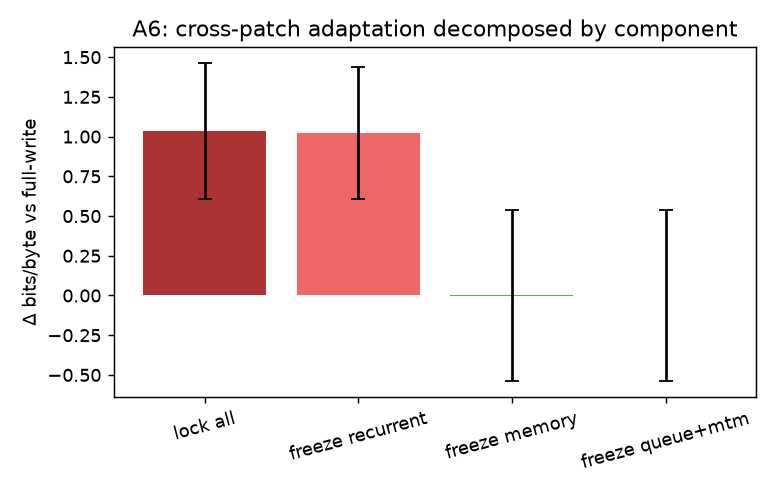
\includegraphics[width=\linewidth]{fig_a6_component_freeze.png}
\caption{A6：跨 patch 适应按组件分解（16\,KB，2 个 seed，误差棒为 95\% CI）。
冻结 \texttt{recurrent} 的代价与冻结全部写入几乎相同；冻结矩阵记忆与队列 $+$ MTM 的代价为零。}
\label{fig:a6}
\end{figure}

\textbf{判定（本文最强的一条归因结论）。}自然文本上的跨 patch 适应\textbf{几乎全部由
\texttt{recurrent}（块级循环状态 \texttt{c\_state}）承担}——
A2（全锁 $+1.00\bits$）、A6（冻结 \texttt{recurrent} $+1.02\bits\approx$ 全锁 $+1.03\bits$）、
A5（边界冲击 $+0.38/0.45\nats$）三个独立实验交叉一致，$4$ 个数量级的不同干预给出同一个答案。
\textbf{这修正了「memory 管长期」的朴素假设}：矩阵记忆在 3\,KB--16\,KB 尺度上是
「一个 patch 即可重建」的快权重，它的价值不在增量适应——冻结其写入几乎零代价，
但它\textbf{读取训练先验}的贡献巨大（去掉热启动后损失升高 $3.7\bits$ 以上，\S\ref{sec:a1}）。
B2-freeze（\S\ref{sec:b2}）在长程复现任务上给出同一归属结论。
\draftnote{版本注：以上归因在 v\_0d3 检查点上测得，其时 \texttt{memory} 跨流共享；
v\_0d4 将其改为序列级私有槽位（\S\ref{sec:model}），「重置 \texttt{memory} $=$ 换共享快照」
的干预语义随之变为「换单流快照」，换用 v\_0d4 检查点后该结论需重新验证。}

\subsection{小结：S1 成立}\label{sec:s1-summary}

\emph{S1 成立}：热启动显著优于空白（$3.73\bits$，同窗口、无收敛趋势），
正常写入显著优于 $\mathit{lock}$（$+1.00\pm0.09\bits$，且随长度累积），两条成立条件同时满足。
归因层面：跨 patch 的信息传递与适应主要由 \texttt{recurrent} 承载，
\texttt{memory} 的作用是\textbf{读取训练稳态先验}，\texttt{queue+MTM} 在本文的尺度上未显示出可测贡献。

\section{实验二：有效上下文窗口（子主张 S2）}\label{sec:s2}

本章用三把尺测量固定状态在损失上等效的上下文长度：位置衰减（\S\ref{sec:b1}）、
重复距离（\S\ref{sec:b2}）、等效滑窗（\S\ref{sec:b3}），外加精确检索的边界预实验（\S\ref{sec:b4}）。
截至本稿，前两把尺已完成（其中位置衰减以单流曲线替代），后两者未完成，如实标注。

\subsection{长文档位置衰减（B1）}\label{sec:b1}

\textbf{做成了什么。}完整的 B1（$5$--$10$ 篇 3 万--10 万字节文档的整篇曲线）尚未运行；
作为替代，本文已有两条\textbf{单流逐 patch 曲线}：96\,KB（seed 7）与 512\,KB（seed 11），
并在同一条流上做了重置频率扫描（E5）。

\textbf{结果（图 \ref{fig:e1} 右、图 \ref{fig:e5}）。}
96\,KB 流上逐 patch NLL 从前段 $0.4970$、中段 $0.6238$ 漂移到后段 $0.7784\nats$；
512\,KB 流同形状（$0.695\to0.874\nats$），全程无尖峰。
重置频率扫描（64\,KB 文本，状态每 $N$ token 重置回热启动快照，$N\in\{512,4096,16384,\infty\}$）
给出 $1.2147/1.0611/1.0430/1.0385\bits$——\textbf{单调下降、无 U 形}。

\begin{figure}[H]
\centering
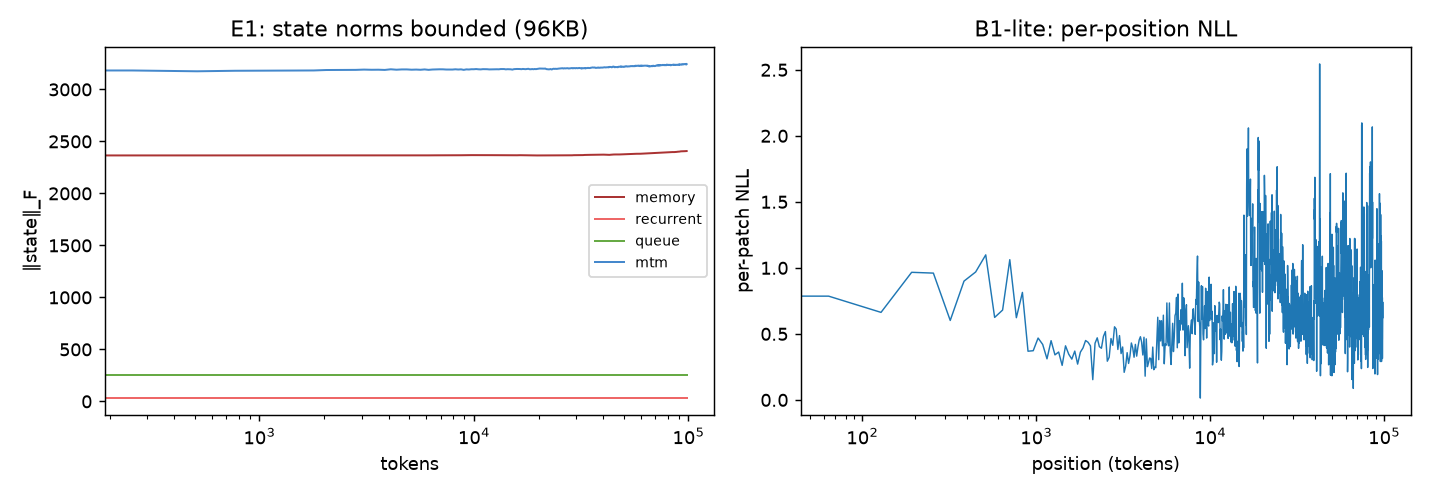
\includegraphics[width=\linewidth]{fig_e1_norms.png}
\caption{E1：96\,KB 单流的状态范数与逐 patch NLL。左：四分量范数（对数横轴）全程有界；
右：per-position 曲线（B1-lite），后段抬升与文本难度漂移一致（由 E5 判定，见正文）。}
\label{fig:e1}
\end{figure}

\begin{figure}[H]
\centering
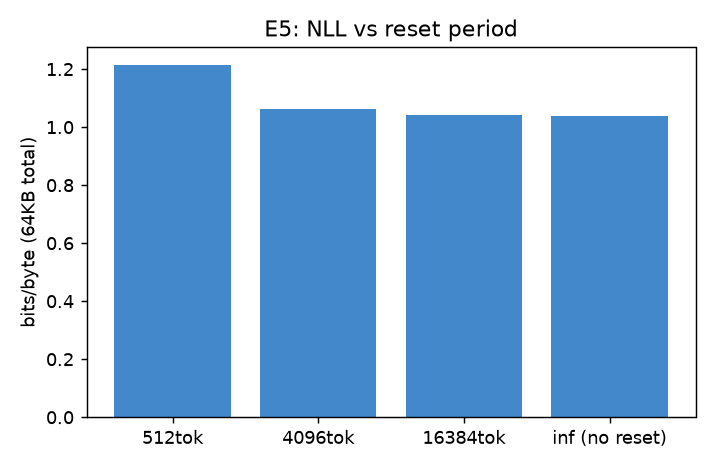
\includegraphics[width=0.62\linewidth]{fig_e5_reset.png}
\caption{E5：64\,KB 文本上，状态每 $N$ token 重置一次的总 bits/byte。
单调下降、无最优重置点 $\Rightarrow$ 在这个尺度上「永续写入」是纯收益、没有噪声累积。}
\label{fig:e5}
\end{figure}

\textbf{判定。}后段 NLL 的抬升\textbf{不是状态退化}：若存在噪声累积，重置频率扫描应出现 U 形
（重置太少则累积过噪声、太多则丢信息），而实测是单调的——每多写一点就多赚一点。
因此该抬升更保守的解释是流内文本难度/分布的漂移。这一点必须在论文里写清，
因为它决定了「永续写入」是否安全。\pending{B1 的整篇 vs 切段对照（真曲线）待补：
需要 5--10 篇长文档，实现见《论文大纲-B》第 3 章第 3.1 节。}

\subsection{自然重复的携带距离（B2）}\label{sec:b2}

\textbf{设计（免合成）。}在同一份 held-out 上流式取逐字节 NLL，扫描流内 $\mathrm{n}$-gram
（$n=8,16$）的第二次出现，按与第一次出现的距离分桶
（$<\!1$k / $1$k--$4$k / $4$k--$16$k / $16$k--$64$k / $>\!64$k 字节），
每个 gram 只计首次复现，指标为两次出现处 $\mathrm{n}$ 个字节 NLL 的均值（nats），
增益 $=$ 首次 $-$ 二次。

\textbf{结果（表 \ref{tab:b2}、图 \ref{fig:b2}）。}96\,KB 流、$n=8$：
增益\textbf{集中在 $<\!1$k 桶（$+0.0839\nats$，9384 对）}，
$1$k--$4$k 桶降至 $+0.019$，$4$k 以外为 $-0.013/-0.030/-0.015$；
$n=16$ 同形状（$<\!1$k 桶 $+0.0797$），但远桶样本数只有 $38/21$，噪声大。
512\,KB 流上 $<\!1$k 桶增益 $+0.0668\nats$（49716 对），
$1$k--$4$k 桶为 $-0.005$，$64$k--$256$k 与 $>\!256$k 桶分别在 $+0.006/-0.013$ 附近波动（图 \ref{fig:e1long} 右）。

% B2：自然重复距离分桶
\begin{table}[t]
\centering
\caption{B2 自然重复的复现距离分桶（96\,KB 流，$n=8$；已按修复后的分桶实现重跑）。
「距离」为与首次出现之间的字节距离（本模型中字节即 token）；
增益 $=$ 首次 $-$ 二次，正值表示第二次出现被更好地预测。
样本数互不相同这一点是分桶正确性的必要条件（见正文勘误说明）。
bucket 间比较并非完全受控——不同距离上重复的是不同的 $\mathrm{n}$-gram 群体，其首次出现难度本身不同。}
\label{tab:b2}
\small
\begin{tabular}{@{}lccccc@{}}
\toprule
距离桶 & $<\!1$k & $1$k--$4$k & $4$k--$16$k & $16$k--$64$k & $>\!64$k \\
\midrule
配对数量（$n=8$） & 9384 & 1225 & 1309 & 2708 & 382 \\
首次出现 NLL (nats) & $0.6863$ & $0.5167$ & $0.4773$ & $0.4665$ & $0.5082$ \\
二次出现 NLL (nats) & $0.6024$ & $0.4977$ & $0.4900$ & $0.4964$ & $0.5229$ \\
\midrule
\textbf{增益 (nats)} & $\mathbf{+0.0839}$ & $+0.0191$ & $-0.0127$ & $-0.0299$ & $-0.0148$ \\
\midrule
\multicolumn{6}{@{}l}{$n=16$（配对数量 3712 / 244 / 38 / 243 / 21）：增益 $+0.0797$ / $+0.0054$ / $-0.0467$ / $-0.0042$ / $+0.0021$} \\
\bottomrule
\end{tabular}
\end{table}


\begin{figure}[t]
\centering
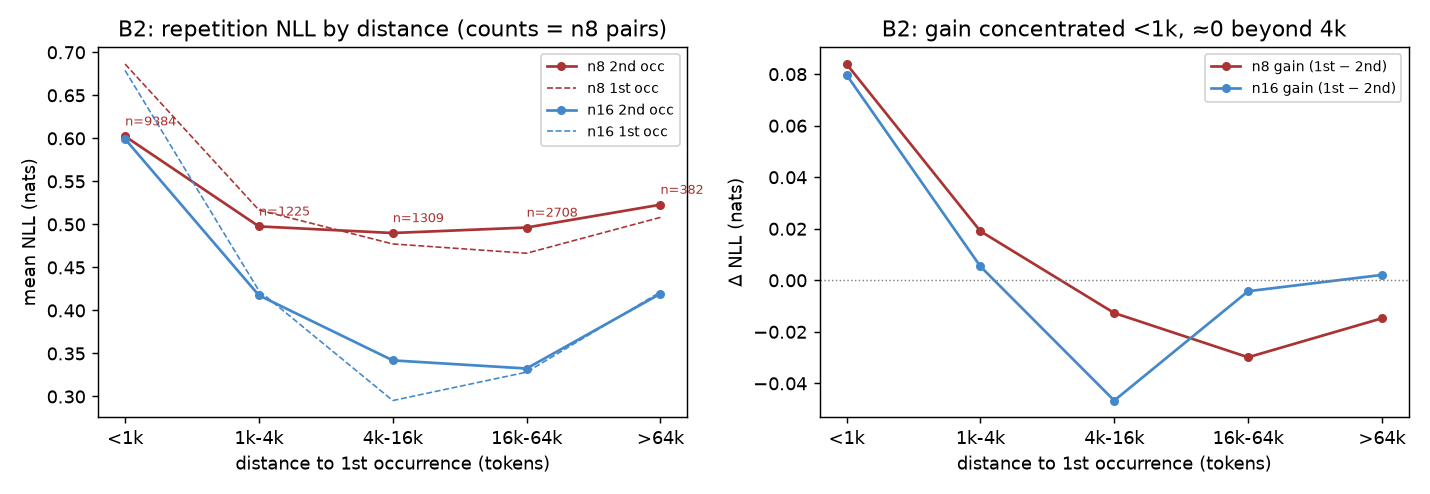
\includegraphics[width=\linewidth]{fig_b2_repetition.png}
\caption{B2：自然重复的复现 NLL 与距离（96\,KB 流）。
左：两桶的首次/二次出现 NLL（标注 $n=8$ 的配对数量）；
右：增益 $=$ 首次 $-$ 二次。增益集中在 $<\!1$k，$4$k 之外衰减到零甚至转负。}
\label{fig:b2}
\end{figure}

\textbf{组件归属（B2-freeze）。}把同一份 96\,KB 文本分别跑 5 个条件（全写、全程只读、冻结单分量），
$<\!1$k 桶增益为：write $+0.0839$、lock $-0.0050$、freeze \texttt{memory} $+0.0840$、
\textbf{freeze \texttt{recurrent} $-0.0043$}、freeze \texttt{queue}$+$\texttt{MTM} $+0.0837$
（表 \ref{tab:attr}(b)、图 \ref{fig:b2freeze}）。
\textbf{冻结 \texttt{recurrent} 精确抹平了复现增益}，代价层面也与全程只读等价
（bits/byte $2.153$ 对 $2.164$）。
这与 \S\ref{sec:s1-attr} 的 A6 结论自洽：该记忆存在 \texttt{recurrent} 里且是写入依赖的。

\begin{figure}[H]
\centering
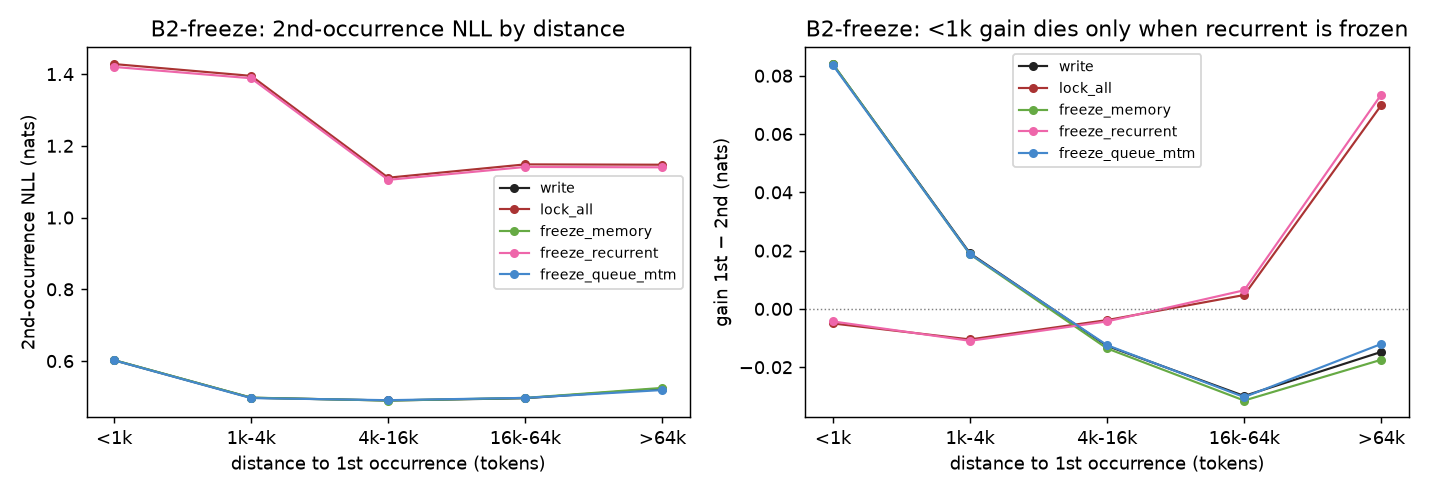
\includegraphics[width=\linewidth]{fig_b2_freeze.png}
\caption{B2-freeze：复现记忆的组件归属。左：二次出现的 NLL 曲线（5 个条件）；
右：增益 $=$ 首次 $-$ 二次。只有 \texttt{recurrent} 被冻结（或全程只读）时 $<\!1$k 增益消失，
冻结矩阵记忆与队列 $+$ MTM 无损。}
\label{fig:b2freeze}
\end{figure}

\textbf{一处必须公开的勘误。}早期版本曾得到「复现增益在 $<\!1$k 到 $>\!256$K 的所有距离桶内
零衰减」的结论，并据此写了「固定状态的记忆 $\ge256$K token 不衰减」。该结论\textbf{作废}：
分桶统计的实现把各桶的样本数写成了同一个值（每桶的数值被复制成同一份），
即「零衰减」是\textbf{所有桶都在报告同一个桶}造成的假象。
修复后重跑（96\,KB 与 512\,KB 两条流）即得到上表结果。
本文所有 B2 数字均为修复后数值；受影响的三张图已重画。
\textbf{教训}：分桶类统计必须在脚本里断言「各桶样本数互不相同且总和等于配对总数」，
否则一个变量作用域缺陷就会产出看起来干净、实则自证的曲线。

\begin{figure}[t]
\centering
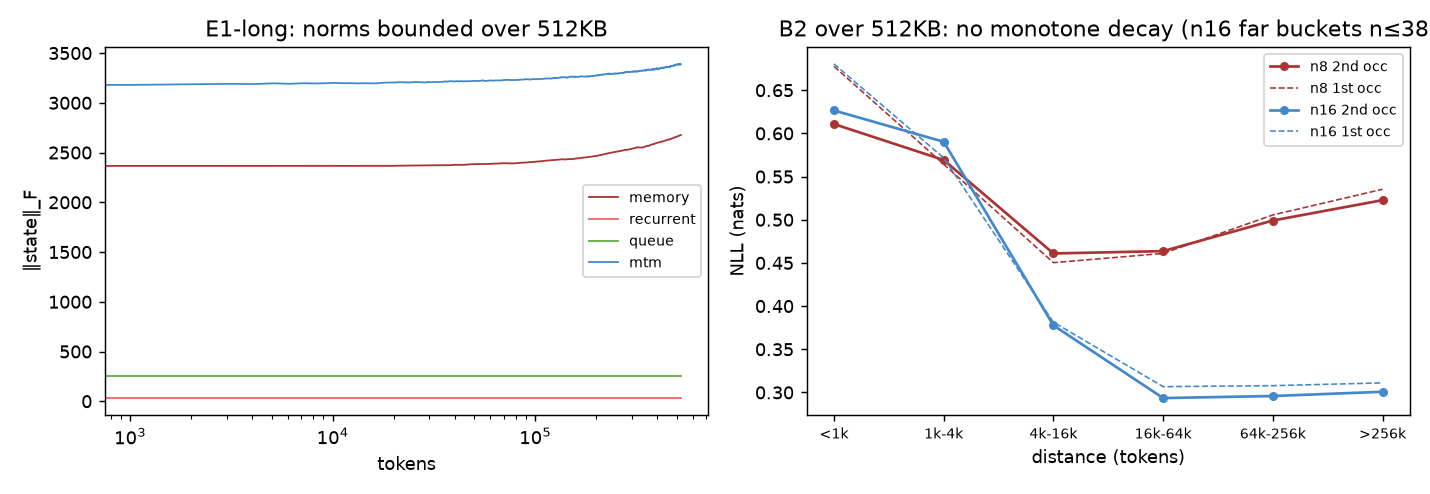
\includegraphics[width=\linewidth]{fig_e1long_b2.png}
\caption{E1-long：512\,KB 单流。左：状态范数（memory $\times1.13$、MTM $\times1.07$，STM/queue 恒定）；
右：B2 距离分桶的首次/二次出现 NLL——无单调衰减形状，$n=16$ 的远桶样本数 $\le1294$，读图需谨慎。}
\label{fig:e1long}
\end{figure}

\textbf{判定。}S2 的量化结论是：固定状态的\textbf{有效重复记忆距离约为 $1$--$4$k token}
（$<\!1$k 内增益显著，$4$k 外基本消失），且这一记忆\textbf{完全由 \texttt{recurrent} 承载}。
一个自洽的旁证：模型内部的通量结构里，队列的时标是 $64$ 槽 $\times$ $64$ token $=4096$ token
（表 \ref{tab:state}），与实测的 $1$--$4$k 量级吻合。\pending{该「时标吻合」是否有因果含义，
需要 C 线（受控注入 + 组件分离的遗忘曲线）才能判定，见附录 \ref{app:c1}。}

\subsection{等效滑窗基线（B3）}\label{sec:b3}

\textbf{设计（未完成）}：训一个 $2$--$4$ 层、局部因果窗口为 $W$ 的 byte Transformer 基线
（$W\in\{512,2\mathrm{k},8\mathrm{k},32\mathrm{k}\}$，数据同分布），
在 B1 的同一批长文档上跑同一套 teacher-forced 循环，得到各档 $W$ 的逐位置曲线，
对每个位置插值出与固定状态曲线最接近的 $W$，即「固定状态 $\approx W$ token 滑窗」的等效窗口。
来不及训练时的降级方案是引用公开滑窗基线并注明口径差异。
\pending{本项需要训练基线，超出「只用现成权重」的范围；这也是本文唯一能给出 S2 绝对数字的途径。}

\subsection{精确检索的边界（B4）}\label{sec:b4}

\textbf{设计（未完成）}：在距离 $d\in\{1\mathrm{k},4\mathrm{k},16\mathrm{k}\}$ 处插入 \texttt{key: value}，
文末 probe，统计精确匹配率。
\textbf{先行证据（指向「不擅长」）}：合成任务上的离散绑定测试（附录 \ref{app:g}）
显示该检查点对随机 ASCII 键值对的绑定很弱——
$k$ 次演示后答案位 NLL 仍在 $8.3$--$8.6$ bits（机会线 $8.23$），$k$ 增大不累积；
换成分布内的词对后曲线完全平（$5.0$--$5.2$ bits，与首字节机会线重合），
即这不是合成数据 OOD 造成的。据此本文\textbf{预判 needle 类精确检索不是本架构的强项}，
将其降级为限定 claim 与未来工作（\S\ref{sec:limits}），并如实报告而不是回避。

\subsection{小结：S2 部分成立}\label{sec:s2-summary}

\emph{S2 的部分结论}：有效窗口\textbf{显著大于 0}（$<\!1$k token 内复现增益 $+0.084\nats$、
且 $1$k--$4$k 仍有残余），但\textbf{远小于}早期误导性结论给出的 $\ge256$K：
固定状态在这个检查点上的自然重复记忆距离是 $1$--$4$k token。
因此「永续上下文」这一强主张\textbf{在当前证据下不成立}，
可辩护的表述是「固定大小状态等效于一段数 k token 的滑动记忆，且其容量不随历史增长而衰减」。
稳定性侧的正面证据（$512$\,KB 连续写入范数有界、重置频率扫描单调）说明\textbf{长度}不是问题，
瓶颈在\textbf{容量与写入/读出机制}——这正是下一步训练侧实验（F 线）要回答的问题（\S\ref{sec:discussion}）。

\section{讨论}\label{sec:discussion}

\subsection{两个子主张的回答汇总}\label{sec:disc-summary}

表 \ref{tab:summary} 把 S1 / S2 与本文全部证据对上。
一句话总结：\textbf{固定大小的持续状态确实承载了可测的跨上下文信息（S1 成立），
但它的有效记忆距离只有 $1$--$4$k token（S2 部分成立）}；
而这两件事的承载者都是块级循环状态，不是那个参数量最大的矩阵记忆。

% 7.1 汇总表：子主张 × 证据 × 图表 × 判定
\begin{table}[H]
\centering
\caption{S1 / S2 的判定汇总。每个判定句都由对应小节的末句直接给出，可逐条回查。}
\label{tab:summary}
\small
\begin{tabular}{@{}p{0.10\linewidth}p{0.30\linewidth}p{0.43\linewidth}p{0.10\linewidth}@{}}
\toprule
子主张 & 证据（实验） & 关键数字 & 判定 \\
\midrule
S1（有没有） &
A1 热启动 vs 空白 &
同窗口 $1.588$ vs $5.319\bits$（差 $+3.731$），窗口内无收敛趋势 &
\textbf{成立} \\
\addlinespace[2pt]
S1（有没有） &
A2 写入 vs $\mathit{lock}$ &
成对差 $+0.999\pm0.095\bits$；差值前段 $0.585\to$ 后段 $0.771\nats$ &
\textbf{成立} \\
\addlinespace[2pt]
S1（谁承载） &
A5 单组件重置 / A6 冻结 / B2-freeze &
冻结 \texttt{recurrent} $+1.022\bits$（$\approx$ 全锁 $+1.034$）；冻结 \texttt{memory} $-0.0005$；
边界冲击 $0.378/0.450\nats$ &
跨 patch 适应由 \texttt{recurrent} 承载 \\
\addlinespace[2pt]
S2（有多少） &
B1-lite + E5 重置频率 &
96/512\,KB 漂移无尖峰；重置周期 $512\to\infty$：$1.2147\to1.0385\bits$ 单调 &
长度非瓶颈 \\
\addlinespace[2pt]
S2（有多少） &
B2 距离分桶 + B2-freeze &
$<\!1$k 增益 $+0.0839\nats$（9384 对），$4$k 外 $\approx0$；冻结 \texttt{recurrent} 抹平增益 &
\textbf{有效记忆 $\approx1$--$4$k token} \\
\addlinespace[2pt]
S2（折算窗口） &
B3 等效滑窗基线 &
\pending{未完成} &
待定 \\
\addlinespace[2pt]
边界能力 &
B4 needle 预实验 / G1 合成绑定 &
合成键值对绑定弱（$8.3$--$8.6$ bits $\approx$ 机会线） & 限定 claim（\S\ref{sec:limits}） \\
\midrule
评测去污染 &
D2b 成员推断 &
状态级样本记忆 $-0.714\bits$；热启动 train gap $-0.350\pm0.200$，空白 $+0.365\pm0.828$ &
\textbf{主表须双报起点状态} \\
\bottomrule
\end{tabular}
\end{table}


\subsection{设计启示：状态接口的可操纵性}\label{sec:disc-design}

本文所有实验的旋钮都落在架构暴露的接口上，没有一处需要改权重、改数据或改提示词。
这一点的工程含义值得单独记下来：

\begin{itemize}\itemsep3pt
\item \textbf{$\mathit{lock}$ 天然给出受控对照}：因为首个 patch 的输出与正常前向逐位一致
（此时尚未发生写入），两组条件在第一步严格相同，差异只能来自后续的写入行为——
这比「同一模型跑两次但初始化不同」之类的对照干净得多。
\item \textbf{状态不可变 $\Rightarrow$ 实验可并行、可回滚}：每个 patch 后拿到的是新状态对象，
因此可以在同一条快照上同时开出「只重置 \texttt{memory}」「只清零 \texttt{recurrent}」
「冻结 \texttt{queue}$+$\texttt{MTM}」等多个分支而不互相污染。
\item \textbf{组件粒度可到下界}：把「跨 patch 写入」这一整块干预拆成四个分量版本后，
归因结论直接落在分量上（\S\ref{sec:s1-attr}）——
这在 RNN 的隐状态上看不到，因为隐状态没有暴露「按分量置换」的接口。
\end{itemize}

\textbf{代价与纪律}：状态跑一次就变，任何复用都会造成实验间污染；
因此每次评测必须先克隆，且快照必须落盘（本架构的状态一旦被改写无法复原）。

\subsection{与其他实验线的关系与展望}\label{sec:disc-rest}

\subsubsection{状态里装的是什么（D 线）}\label{sec:dline}

A1 说明热启动状态很值钱（$3.73\bits$），D 线回答它值钱在哪里（表 \ref{tab:d1}）。
四个文本档上的 gain（空白 $-$ 热启动）为：\textbf{同分布} $+5.061\pm0.580$、
\textbf{跨域}（sft 尾部）$+4.373\pm0.912$、\textbf{同分布但字节打乱} $-0.314\pm0.331$、
\textbf{零信息}（全空格）$+2.688$（图 \ref{fig:d1}）。
解读：热启动记忆的主体是\textbf{通用序列先验}（跨域仍保留 $\sim4.4\bits$），
叠加少量\textbf{同分布偏向}（$\sim0.7\bits$）；对打乱字节没有先验，
说明记忆锚定的是自然语言的\emph{结构}而不是字节取值本身。

% D1 / D2 / D2b：热启动记忆的性质
\begin{table}[t]
\centering
\caption{D 线：热启动状态里装的是什么（4\,KB $\times$ 5 seed，95\% CI）。
（a）D1 领域分解：gain $=$ 空白 $-$ 热启动，四档文本；
（b）D2/D2b 成员推断：训练消费区 vs 未消费同分布文本，以及「去掉热启动」后的同一比较。
热启动的收益主要是通用序列先验（跨域仍在），含少量同分布偏向；
而\textbf{逐样本的训练痕迹几乎全部由状态承载}（去掉热启动后 train gap 消失）。}
\label{tab:d1}
\small
\begin{tabular}{@{}lccc@{}}
\toprule
\multicolumn{4}{@{}l}{\textbf{(a) D1 四档文本（4\,KB $\times$ 5 seed）}} \\
\midrule
文本档 & 热启动 (bits/byte) & 空白 (bits/byte) & gain（空白 $-$ 热启动） \\
\midrule
同分布 held-out & $1.323\pm0.239$ & --- & $+5.061\pm0.580$ \\
跨域（sft 尾部） & $1.681\pm0.081$ & --- & $+4.373\pm0.912$ \\
同分布但字节打乱 & $11.901\pm0.463$ & --- & $-0.314\pm0.331$ \\
零信息（全空格） & $0.236$ & --- & $+2.688$ \\
\midrule
\multicolumn{4}{@{}l}{\textbf{(b) D2 / D2b 成员推断}} \\
\midrule
条件 & 消费区 (bits/byte) & 未消费 (bits/byte) & gap（消费 $-$ 未消费） \\
\midrule
热启动（权重 $+$ 状态） & $0.973\pm0.173$ & $1.323\pm0.239$ & $-0.350\pm0.200$ \\
空白（仅权重） & --- & --- & $+0.365\pm0.828$ \\
\midrule
\multicolumn{4}{@{}l}{状态级样本记忆 $=$ 热启动 gap $-$ 空白 gap $= \mathbf{-0.714}$ bits/byte} \\
\bottomrule
\end{tabular}
\end{table}


\begin{figure}[t]
\centering
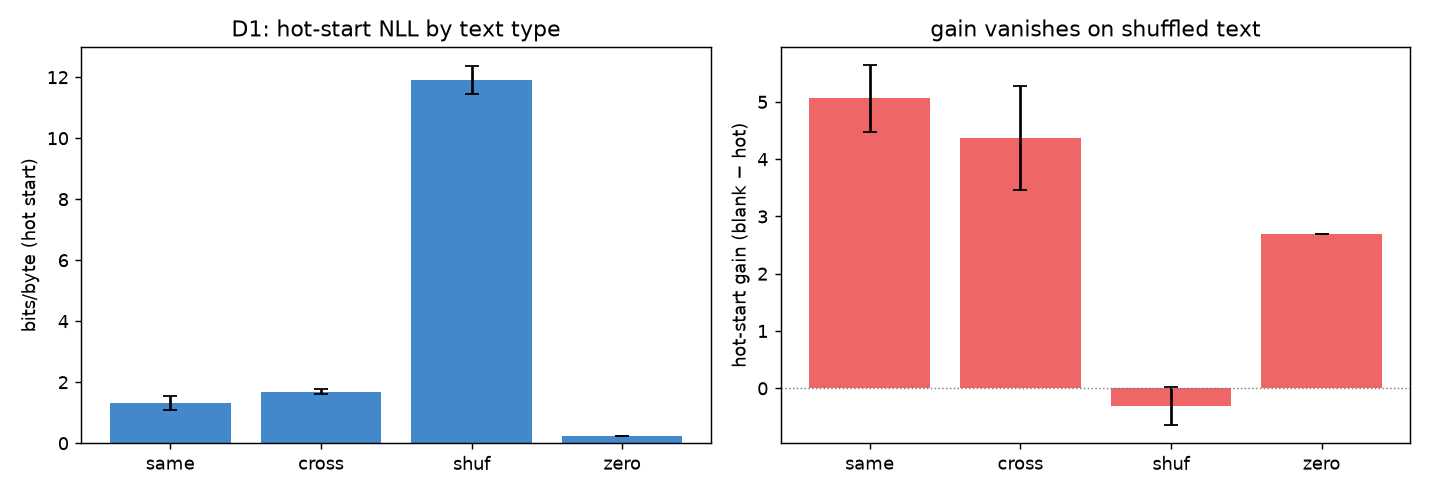
\includegraphics[width=\linewidth]{fig_d1_domain.png}
\caption{D1：热启动记忆的领域分解（4\,KB $\times$ 5 seed）。左：各档文本的热启动 NLL；
右：gain（空白 $-$ 热启动）——跨域仍保留大部分收益，打乱字节的收益为负。}
\label{fig:d1}
\end{figure}

\textbf{成员推断（D2 / D2b）是必须公开的一条。}训练消费区文本在热启动下的 NLL 比未消费同分布文本低
$-0.350\pm0.200\bits$；把起点换成空白后这个差距消失（$+0.365\pm0.828$，与 0 无显著差异），
反推\textbf{状态级样本记忆} $=-0.714\bits$。也就是说：\emph{逐样本的训练痕迹几乎完全由状态承载，权重没有贡献}。
两个含义：其一，评测协议上任何用热启动的数字都带着「这几段文本模型可能见过」的脚注，
主表必须双报起点状态（\S\ref{sec:cond}）；其二，隐私与去污染上，状态本身是记忆载体，
这不只是统计压缩问题。

\subsubsection{超长上下文的数值安全（E 线）}\label{sec:eline}

96\,KB 单流：$\|\texttt{memory}\|_F\times1.018$、$\|\texttt{MTM}\|_F\times1.019$，
\texttt{recurrent}/\texttt{queue} 范数构造性恒定；
512\,KB 单流：$\times1.132$ 与 $\times1.065$（图 \ref{fig:e1} 左、图 \ref{fig:e1long} 左）。
全程有界缓增、未见发散——这是 delta 规则 $+$ $1/\mathrm{eff\_seq\_len}$ 门控在数值上的正面证据。

\textbf{污染与自愈（E2）}：正常 8\,KB $+$ 随机字节 4\,KB $+$ 正常 8\,KB 的流上，
污染段内的 NLL 冲击为 $+9.25$（照常写入）与 $+9.92\nats$（污染段设为只读）；
但\textbf{两组条件的尾部 NLL 只差 $0.0001$}（$0.8608$ vs $0.8607$），残留都是 $+0.085\nats$。
结论有两层：污染写入只造成\textbf{瞬时冲击}（污染后头 4 个 patch：$0.686$ vs $0.436\nats$），
\textbf{没有长期残留}；也因此「只读模式可作污染防御」这一说法\textbf{得不到数据支持}——
残留量在两个条件下相同，尾部抬升更可能来自文本难度变化（与 \S\ref{sec:b1} 的漂移解释一致）。
图见附录 \ref{app:eline}。

\subsubsection{前向学习：连续适应而非离散绑定（G 线）}\label{sec:gline}

持续状态的另一面是「读着读着就变了」。合成任务上的结果（附录表 \ref{tab:g}、图 \ref{fig:g1}、\ref{fig:g1c}）
可以概括为一句话：\textbf{这个检查点上的前向学习是连续适应，而不是离散绑定}。
（i）随机 ASCII 键值对联想：$k$ 次演示后 write 条件仍在 $8.3$--$8.6$ bits
（机会线 $8.23$），且不随 $k$ 累积；write 与 $\mathit{lock}$ 的差只有 $+0.37$--$+0.66\bits$。
（ii）把符号换成分布内高频词对后曲线\textbf{完全变平}（$5.0$--$5.2$ bits，与首字节机会线重合），
说明这\textbf{不是}合成数据 OOD 造成的——是 delta 规则通道对离散配对的绑定本身很弱。
（iii）自然语料上的 $8$-gram 复现增益只有 $+0.054\nats$，且在 $\mathit{lock}$ 下消失。
把这三条与 A2/A6 的 $+1.00\bits$ 放在一起看，\textbf{跨 patch 的收益主要来自连续的话题/句法适应，
而不是「记住若干条事实」}。这既是本文的机制结论，也是把 needle 类精确检索降级为限定 claim 的直接理由（\S\ref{sec:b4}）。

\subsubsection{下一步：训练侧实验（F 线）}\label{sec:f-line}

本文的全部证据都指向同一个未解问题：为什么有效记忆只有 $1$--$4$k token？
是\textbf{机制上界}（固定状态在这个写入规则下就只能记这么久），
还是\textbf{训练进度}（该检查点只训到 20\%，长程写入尚未学出来）？
这需要训练侧实验才能分辨，按优先级：

\begin{enumerate}\itemsep3pt
\item \textbf{BPTT 窗口扫描}（$\mathrm{bptt}=1/4/8$）：$\mathrm{bptt}=1$ 时梯度只到 patch 内，
长程信用\textbf{只能}经前向 delta 规则传递。它的长程表现保留多少，
即「前向通道」的贡献上限；$1\to4$ 的增益即梯度通道的贡献。
这是本文「持续学习」主张在训练侧的判决性实验。
\item \textbf{永续 vs 文档边界重置训练}：直接检验「训练时不清状态到底是收益还是负担」。
\item \textbf{状态收敛（F5）}：用早期/中期/晚期检查点比较热启动收益与状态间相似度，
回答「热启动之所以有效」的前提是否稳定。
\item \textbf{chunk\_size（并行流数）扫描}：v\_0d3 中 \texttt{memory} 的写入是跨流平均的，
流数直接改变「每流写入占比」；v\_0d4 改为序列级私有槽位后，流数变为「独立记忆实例数」，
该扫描在两版语义下问的是不同的问题——与推理 batch$=1$ 的匹配度直接相关。
\end{enumerate}

在这些实验完成之前，本文的结论应当被理解为\textbf{该检查点在该规模上的实测上界}，
而不是该架构的能力上界。

\section{局限与结论}\label{sec:limits}

\subsection{局限}\label{sec:limitations}

\textbf{（1）单一检查点、单一规模，且只训练到 20\%。}本文全部数字来自
\texttt{gridman\_medium\_v\_0d3\_pretrain}（437.8M 参数，step $144{,}000/705{,}600$），
没有验证集、没有同预算基线（\S\ref{sec:b3} 未完成）。
因此：绝对值（如 $1.08\bits$）\textbf{不可}与任何外部模型对照，
所有结论只在\textbf{条件间}成立；「有效记忆 $1$--$4$k token」也\textbf{不能}排除
「换个训练更充分的检查点会显著更长」的可能。加验证集、训完 medium、补一个同预算的
byte Transformer 基线，是本稿升级为投稿稿的最低条件。

\textbf{（2）精确检索与离散绑定。}合成键值对与词对联想上，本检查点的绑定能力弱到接近机会线
（\S\ref{sec:gline}）；据此本文把 needle 类精确检索降级为限定 claim，
并如实说明「统计/语义级的长程记忆」才是本文证据支持的范围。B4 预实验本身\textbf{尚未运行}。

\textbf{（3）热启动与训练语料的污染边界。}状态级样本记忆 $=-0.714\bits$
说明热启动起点含着训练语料的具体痕迹（\S\ref{sec:dline}）。
本文据此要求主表双报起点状态；但「双报」只解决报告透明，
不解决\textbf{污染本身}——严格版本需要用完全无重叠的评测集重做 A/B/C 三组。
$\mathrm{n}$-gram 重叠率的精确统计 \pending{待补，见附录 \ref{app:decontam}}。

\textbf{（4）受控遗忘曲线缺失。}计划中的 C 线（注入键值对、按距离与组件分解测 recall 衰减）
因实现缺陷作废（附录 \ref{app:c1}），修订版尚未重跑。
这意味着本文\textbf{没有}一条真正受控的遗忘曲线：
\S\ref{sec:b2} 的重复距离是对自然文本的观察性测量，
其各距离桶之间并非完全受控（不同距离上重复的是不同 $\mathrm{n}$-gram 群体，首次出现难度本就不同）。

\textbf{（5）实现版本已演进，部分归因结论绑定旧语义。}本文数字全部出自 v\_0d3 检查点；
现行 v\_0d4 把 \texttt{memory} 改为序列级私有槽位（无跨流平均、无跨卡同步）。
推理侧（$\mathrm{batch}=1$）两版逐位对应，主结论（S1/S2、A1/A2/B2）不受影响；
但\textbf{训练侧语义已变}：v\_0d3 的「重置 memory $=$ 动共享知识」在 v\_0d4 中退化为只影响单流，
\S\ref{sec:s1-attr} 的组件归因、A5 的 memory 回滚语义在 v\_0d4 检查点上需重新验证。
此外 v\_0d3/v\_0d4 存档互不兼容，跨版续训不可行。

\textbf{（6）未完成项。}A4（状态错配）、B3（等效滑窗基线）、B4（needle 预实验）、
F 线（训练侧全部实验）、E3（精度链漂移）、E4（自由运行分叉）均未运行，
正文与附录中一律标注为待补，不以任何形式给出推测数值。

\textbf{（7）口径订正史（主动披露）。}本稿在定稿前对实验包做了逐脚本审读，
修正了三处口径问题（$\mathrm{n}$-gram 分桶缺陷导致的一条错误结论已撤回、
A1 计分窗口未对齐、C1 答案位置偏移导致该实验作废），并补了模型无关的回归自检。
保留这段历史的原因是：其中一条（「长程零衰减」）曾经看起来非常漂亮，
而它恰恰来自一个会让所有桶报告同一份数据的实现缺陷。\textbf{分桶/配对类统计必须断言样本数互不相同}，
这条纪律比结论本身更重要。

\subsection{结论}\label{sec:conclusion}

本文把「固定大小的持续状态能承载多少跨上下文信息」当作一个可测量的经验问题，
在一个 437.8M 参数的 byte 级有状态语言模型上，用 teacher-forced bits/byte 与状态手术
（热启动/空白、commit/$\mathit{lock}$、分量重置/冻结）做了系统消融，得到三条可以直接引用的结论。

\textbf{第一，状态确实在携带信息，且写入有因果贡献。}同一计分窗口下热启动比空白低 $3.73\bits$
且无收敛趋势；锁定跨 patch 写入的代价是 $+1.00\pm0.09\bits$，并随上下文累积。S1 成立。

\textbf{第二，承载者是块级循环状态，不是参数量最大的矩阵记忆。}冻结 \texttt{recurrent}
的代价（$+1.022\bits$）与冻结全部写入（$+1.034\bits$）几乎相同；
冻结 delta 规则矩阵记忆的代价为零（$-0.0005\bits$），
但去掉热启动使损失升高 $3.7\bits$ 以上——\textbf{矩阵记忆的价值在读取训练稳态先验，
不在增量适应}。这个结论由 A2/A5/A6/B2-freeze 四组独立实验交叉支撑。

\textbf{第三，有效记忆距离约为 $1$--$4$k token，且长度不是瓶颈。}自然重复的复现增益集中在
$<\!1$k（$+0.084\nats$），$4$k 之外衰减到零；同时 $512$\,KB 连续写入下状态范数有界
（memory $\times1.13$），重置频率扫描单调无 U 形。因此「永续写入」在数值上是安全的，
瓶颈在容量与写入/读出机制，而不是「能不能一直写下去」。

\textbf{对「永续上下文」主张的净判断}：固定大小状态\textbf{可以}持续携带信息，
并且\textbf{可以}在远长于其有效记忆距离的流上稳定运行；
但在本文这个检查点上，它的记忆能力等效于数 k token 的滑动记忆，
尚不足以支撑「记住了整条流」的强主张。
下一步的判决性实验是 BPTT 窗口扫描（$\mathrm{bptt}=1$ 保留多少长程能力）
与永续 vs 边界重置训练的对照（\S\ref{sec:f-line}）——
前者区分「前向通道上界」与「梯度通道贡献」，后者直接回答「训练时不清状态是收益还是负担」。


\appendix
% 附录 A–F 连续排布，不再每个大标题换页（正文 1–8 仍换页）。
\let\section\origsection
\section{完整实验配置、检查点与复现}\label{app:config}

\footnotesize
\setlength{\tabcolsep}{3pt}
\begin{longtable}{@{}p{0.13\linewidth}p{0.52\linewidth}p{0.27\linewidth}@{}}
\caption{配置与检查点事实。标「推算」的量为本文推算，其余引自团队实现文档与配置。}
\label{tab:config}\\
\toprule
项 & 值 & 备注 \\
\midrule
\endfirsthead
\multicolumn{3}{@{}l}{\tablename~\thetable\ （续）}\\
\toprule
项 & 值 & 备注 \\
\midrule
\endhead
\midrule
\multicolumn{3}{@{}r}{续下页}\\
\endfoot
\bottomrule
\endlastfoot
模型配置 & \texttt{GRIDMAN\_MEDIUM}：\texttt{embed\_dim}=1024，\texttt{blocks}=3，\texttt{patch\_size}=64（本文检查点 v\_0d3：\texttt{chunk\_size}=192；现行 v\_0d4 MEDIUM：\texttt{chunk\_size}=1，\texttt{bptt}=16） & 4 个 \texttt{c\_state} \\
实现版本 & 行为描述 v\_0d4（2026-10-18）；全部数字出自 v\_0d3 检查点，存档不互相兼容 & 见 \S\ref{sec:model} 表 \ref{tab:version} \\
参数量 & 437.8M & 权重 $+$ 状态合计 \\
词表 & 300（字节 0--255，\texttt{pad}=256，\texttt{eos}=257） & byte 级，无 OOV \\
状态规模 & batch$=1$ 切片合计 $14{,}072{,}832$ 个 fp32 元素（$\approx53.7$\,MiB）：\texttt{memory} $12{,}954{,}624$（$49.4$\,MiB）$+$ \texttt{MTM} $1{,}048{,}576$（$4.0$\,MiB）$+$ \texttt{queue} $65{,}536$（$0.25$\,MiB）$+$ \texttt{recurrent} $4{,}096$（$0.016$\,MiB） & 按 v\_0d4 \texttt{StateLayout} 实测 \\
训练 & AdamW $+$ cosine，clip $1.0$，bf16，lr $5\times10^{-4}$，\texttt{bptt}=4 patch（256 token） & 192 条并行永续流（v\_0d3 检查点口径） \\
检查点 & \texttt{gridman\_medium\_v\_0d3\_pretrain}，step $144{,}000/705{,}600$（20\%） & 唯一使用的权重 \\
\midrule
\multicolumn{3}{@{}l}{\textbf{数据}} \\
\midrule
预训练 & \texttt{pretrain.jsonl} $\approx9.5$\,GB，每行 \texttt{\{"text": ...\}} & 每条流 chunk $\approx49.4$\,MB \\
微调 & \texttt{sft.jsonl} $\approx14$\,GB，多轮对话（仅 assistant token 计 loss） & 用作跨域档 \\
已消费区 & 每条流前 $144{,}000\times64\,\mathrm{B}=9.2$\,MB & 推算 \\
held-out 取行 & 每条流 chunk 内偏移 $\ge20$\,MB & 零污染 \\
\midrule
\multicolumn{3}{@{}l}{\textbf{复现：脚本 $\to$ 实验}} \\
\midrule
\texttt{common\_eval.py} & 脚手架：模型单例、teacher-forced 流式评测、文本源、组件手术 & 全部实验共用 \\
\texttt{a1\_hot\_vs\_blank.py} / \texttt{a1\_clean\_heldout.py} & A1（\S\ref{sec:a1}） & 后者为对齐窗口版 \\
\texttt{stage1\_a2\_a3\_a5.py} & A2、A3、A5（\S\ref{sec:a2}、\S\ref{sec:a3}、\S\ref{sec:s1-attr}） & \\
\texttt{stage1b\_a6.py} & A6 组件冻结（\S\ref{sec:s1-attr}） & \\
\texttt{stage2\_d1\_d2.py} / \texttt{stage2b\_d1\_d2.py} / \texttt{stage8\_d2b.py} & D1、D2、D2b（附录 \ref{app:dline}） & 2b 为 5-seed 修订版 \\
\texttt{stage3\_e1\_e5\_b2.py} / \texttt{stage6\_g1c\_e1long.py} & E1、E5、B2（\S\ref{sec:b1}、\S\ref{sec:b2}） & 含 512\,KB 长流 \\
\texttt{stage4\_g1\_g2.py} & G1a、G1b、G2（附录 \ref{app:g}） & \\
\texttt{stage5\_c1\_e2.py} & C1（作废，附录 \ref{app:c1}）与 E2（附录 \ref{app:eline}） & \\
\texttt{stage7\_b2\_freeze.py} & B2-freeze 组件归属（\S\ref{sec:b2}） & \\
\texttt{make\_figures.py} / \texttt{make\_fig\_a1.py} & 全部图表 & \\
\texttt{verify\_positions.py} & 模型无关回归自检（答案位置必须落在自己的 kv 块内） & 无 GPU 也可跑 \\
\end{longtable}
\setlength{\tabcolsep}{6pt}
\normalsize

\section{逐位置完整曲线}\label{app:curves}

正文引用的逐位置曲线：图 \ref{fig:a1}（A1 双曲线 $+$ 差值）、图 \ref{fig:a2}（A2 写入 vs 只读）、
图 \ref{fig:a3}（跨文档边界对齐恢复曲线）、图 \ref{fig:e1}（96\,KB 范数 $+$ per-position）、
图 \ref{fig:e5}（重置频率）、图 \ref{fig:e1long}（512\,KB 范数 $+$ 距离分桶）、
图 \ref{fig:b2} 与图 \ref{fig:b2freeze}（重复距离与组件归属）。
附录 \ref{app:eline} 给出污染自愈曲线（图 \ref{fig:e2}）。

\section{held-out 去污染统计}\label{app:decontam}

本文的 held-out 切分按「每条流 chunk 内偏移 $\ge20$\,MB」取行（\S\ref{sec:data}），
该偏移由「step $\times$ patch 长度 $=$ 9.2\,MB」推算得到，留有 $>2\times$ 余量。
B2 的分桶统计顺带产出了配对数量（表 \ref{tab:b2}），可作为分布性的旁证。
\pending{待补：与训练集（已消费区）的 4-gram 重叠率、以及 $n$-gram 去重后的行级去重率明细；
口径与实现见《论文大纲-B》第 1 章。}

\section{C 线与 E 线：遗忘、污染与稳定性}\label{app:cline}

\subsection{C1 受控遗忘曲线：作废说明}\label{app:c1}

\begin{figure}[H]
\centering
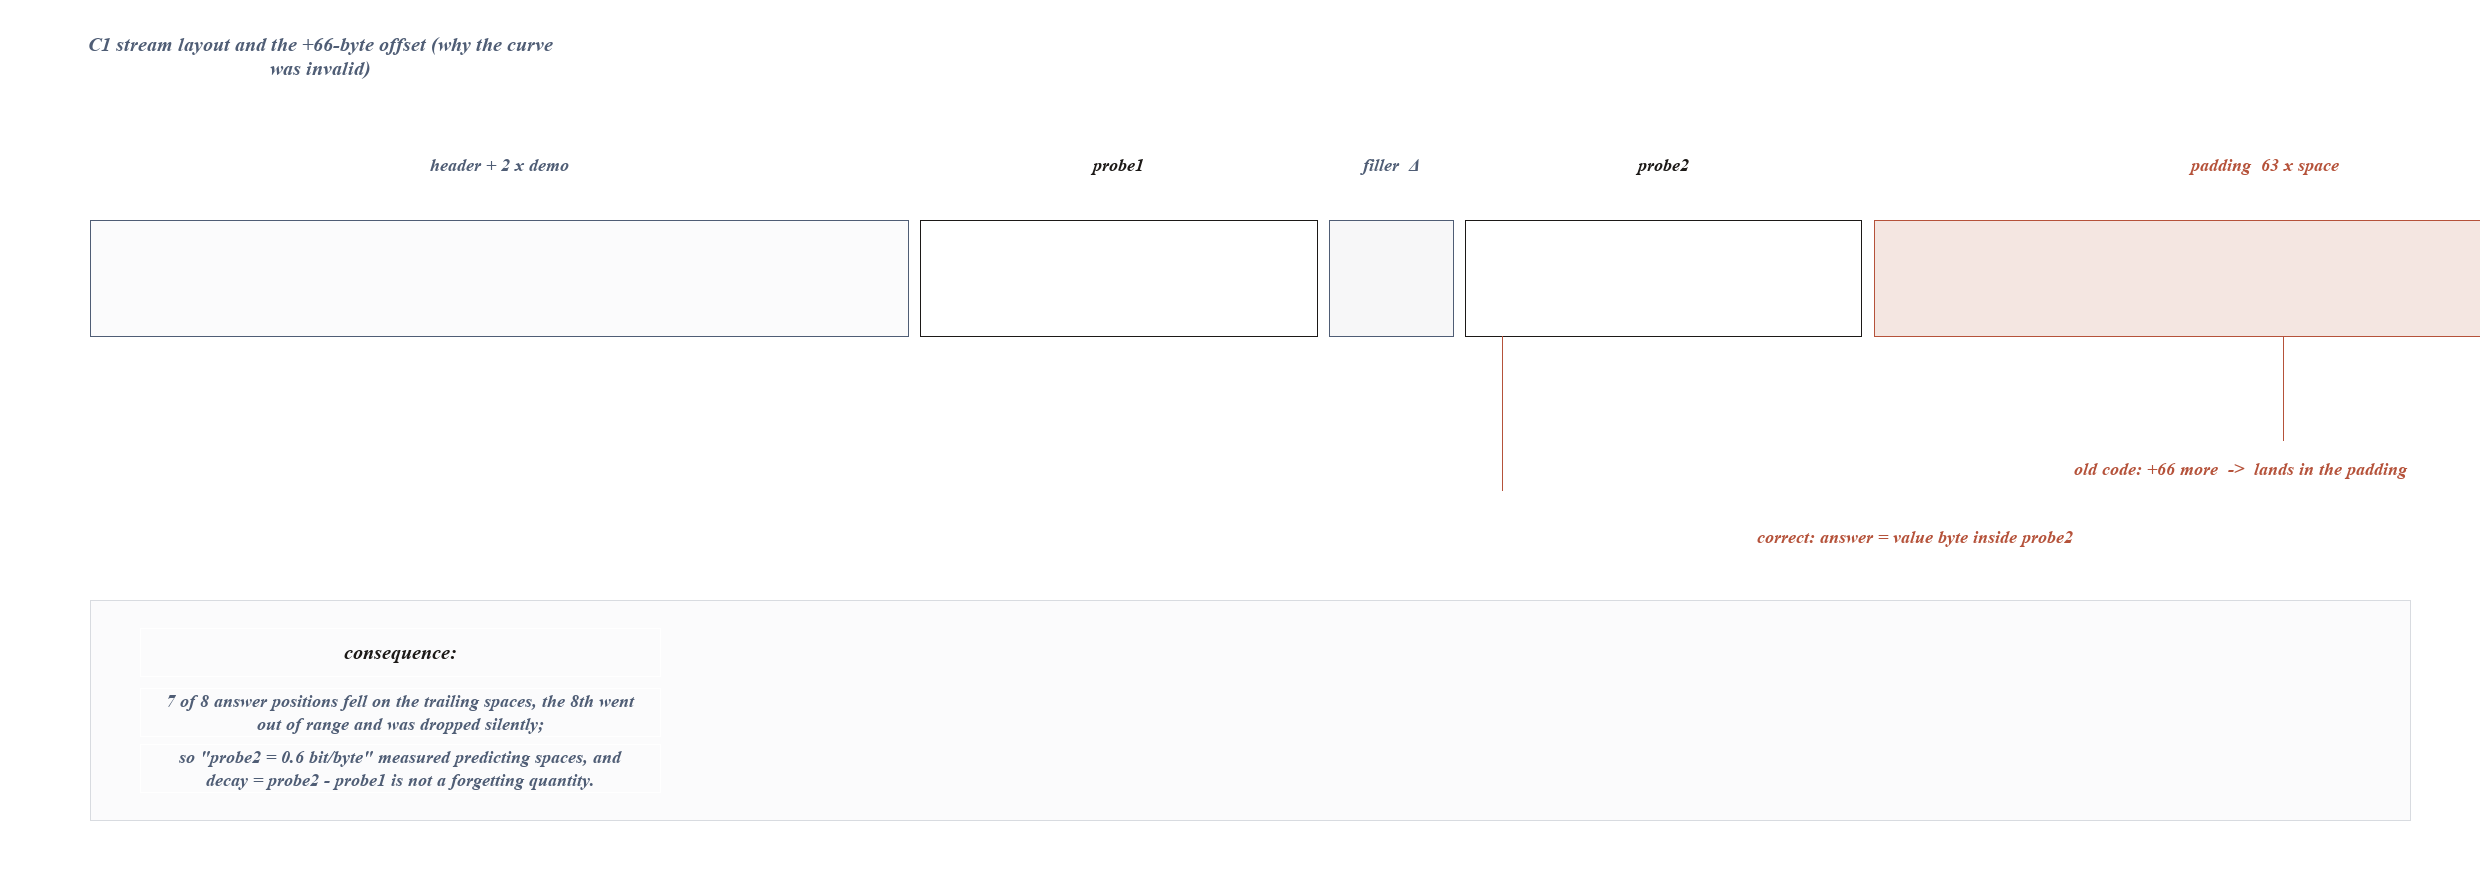
\includegraphics[width=\linewidth]{fig_c1_stream.png}
\caption{C1 的流结构与那 66 字节的偏移（Visio 绘制，源文件 \texttt{figs/fig\_c1\_stream.vsdx}）。
段宽按字节数等比（filler 段压缩），红框为末尾补白；两条竖线分别是「正确答案位置」与「旧代码算出的位置」。}
\label{fig:c1stream}
\end{figure}

\textbf{实验意图。}构造 \texttt{[header $+$ 2$\times$demo $+$ probe1]} $+$ \texttt{filler($\Delta$)}（图 \ref{fig:c1stream}）
$+$ \texttt{probe2} 的合成流（8 对随机 ASCII 键值对、$2$ 次演示），
在 $\Delta\in\{512,2048,8192,32768,131072\}$、$4$ 个条件（正常 / filler 期只读 /
filler 期清零 \texttt{recurrent} / filler 期清零 \texttt{queue}$+$\texttt{MTM}）、$3$ 个 seed 下
测「probe2 相对 probe1 的 recall 衰减」，期望得到按组件分解的遗忘曲线。

\textbf{实测异常。}probe1 的答案位 NLL $=8.38$ bits（机会线 $8.23$），
而 probe2 $=0.6$ bits——\emph{注入后立刻测不会，隔着最多 $128$K token 反而几乎白送}；
四个条件的衰减全挤在 $-7.5$--$-7.8$，彼此不可分。

\textbf{根因（已定位）。}生成脚本把块内偏移基准 $D=\text{header}+2\times\text{demo}=66$ 字节
用在了 probe2 上，而 probe2 的位置又已经叠加了「已注入长度 $+$ $\Delta$」，
于是\textbf{66 字节被算了两次}：8 个答案位置里 7 个落到 probe2 块之后的\textbf{补白空格}上、
第 8 个越界被静默丢弃（代码在位置不在流内时只是跳过）。
所以「probe2 $=0.6$ bits」的真实含义是「模型很会猜一串连续空格」，
而 decay $=$ probe2 $-$ probe1 是伪量。

\textbf{处理。}该实验作废，本文正文不引用其任何数字；
修订版已实现（把「块 $\to$ 答案位置」的算术抽成公共函数，位置一律由「块在流中的绝对起点」推出，
并加断言：答案位置的前一字节必须是 \texttt{=}、后一字节必须是 \texttt{|}），
配套的模型无关自检脚本可在无 GPU 环境下验证位置正确性（旧实现会当场失败）。
\textbf{重跑尚未进行}（预计与原实现同量级，约 80 分钟）。
即使重跑，也需要先注意一个先行事实：本检查点对随机 ASCII 键值对的绑定本身很弱
（附录 \ref{app:g} 的 G1a：$8.3$--$8.6$ bits $\approx$ 机会线），
因此该实验更可能给出「记不住」而不是「记得住但会忘」的结果——
正确的写法是把这类结论归到「离散绑定弱」的机制结论上，而不是包装成遗忘曲线。

\subsection{E2 状态污染与自愈}\label{app:eline}

流结构：正常 8\,KB $+$ 随机字节 4\,KB $+$ 正常 8\,KB；两条件为
\texttt{write\_through}（污染段照常写入）与 \texttt{lock\_garbage}（污染段只读）。
结果见表 \ref{tab:e2} 与图 \ref{fig:e2}：污染段内冲击巨大（$+9.25$ / $+9.92\nats$），
但两组条件的尾值与残留几乎相同（$0.8608$ vs $0.8607$；$+0.085$ vs $+0.085\nats$），
污染后前 4 个 patch 才有明显差异（$0.686$ vs $0.436\nats$）。
\textbf{结论}：污染写入造成瞬时冲击、无长期残留；「只读模式作为污染防御」得不到数据支持。
尾部相对基线的 $+0.085\nats$ 抬升更可能来自文本难度漂移（与 \S\ref{sec:b1} 的 E5 判据一致）。

\begin{table}[H]
\centering
\caption{E2 污染与自愈（nats）。恢复长度按「回到基线 $+0.5$ 以内」判定。}
\label{tab:e2}
\small
\begin{tabular}{@{}lcccccc@{}}
\toprule
条件 & 污染前 & 污染段内 & 污染后 4 patch & 尾部 & 残留 & 恢复（patch） \\
\midrule
write\_through & $0.776$ & $10.027$ & $0.686$ & $0.861$ & $+0.085$ & $0$ \\
lock\_garbage & $0.776$ & $10.696$ & $0.436$ & $0.861$ & $+0.085$ & $0$ \\
\bottomrule
\end{tabular}
\end{table}

\begin{figure}[H]
\centering
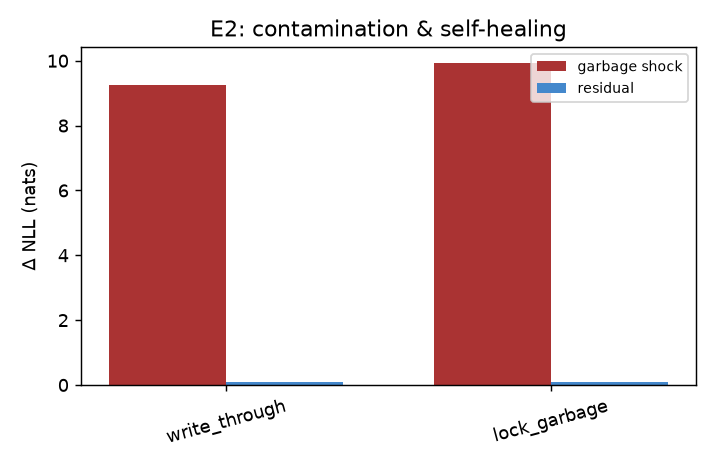
\includegraphics[width=0.62\linewidth]{fig_e2_contamination.png}
\caption{E2：污染段的冲击与残留。冲击量级远大于残留，且两条件的残留相同。}
\label{fig:e2}
\end{figure}

\section{D 线与 G 线的完整数字}\label{app:dline}\label{app:g}

\begin{table}[H]
\centering
\caption{G 线前向学习：合成任务与自然语料。指标为答案位 NLL 的均值（bits），
$5$ 个 seed 的 95\% CI；write / lock 两条件。数值越大越差，机会线见表内注。}
\label{tab:g}
\small
\begin{tabular}{@{}llcc@{}}
\toprule
任务 & 设定 & write & lock \\
\midrule
G1a 随机 ASCII 键值对联想 & $k=0$（无演示） & $8.93\pm0.62$ & $8.93\pm0.62$ \\
（机会线 $\log_2 85\approx6.4$ bits） & $k=1$ & $7.54\pm0.49$ & $7.54\pm0.49$ \\
 & $k=2$ & $8.31\pm0.34$ & $8.98\pm0.65$ \\
 & $k=8$ & $8.53\pm0.61$ & $8.98\pm0.65$ \\
 & $k=16$ & $8.61\pm0.72$ & $8.98\pm0.65$ \\
\midrule
G1b 单字节 bigram 转移 & $k\le8$ & $\approx3.6$--$3.9$ & 同 write \\
（CI 很大，仅定性） & $k=16$ & $3.15\pm1.82$ & $3.91\pm2.21$ \\
 & $k=32$ & $3.33\pm1.96$ & $3.91\pm2.21$ \\
\midrule
G1c 分布内高频词对联想 & $k=0$ & $5.15\pm0.31$ & $5.34\pm0.58$ \\
 & $k=8$ & $4.96\pm0.14$ & $5.17\pm0.30$ \\
 & $k=16$ & $5.19\pm0.12$ & $5.24\pm0.43$ \\
\midrule
G2 自然语料 $\mathrm{8}$-gram 复现 & 首次 / 二次（nats） & $0.732\to0.678$ & $1.483\to1.499$ \\
（32\,KB，3382 对，间距 $<\!4$k） & 增益 (nats) & $\mathbf{+0.054}$ & $-0.016$ \\
\bottomrule
\end{tabular}
\end{table}

\begin{figure}[H]
\centering
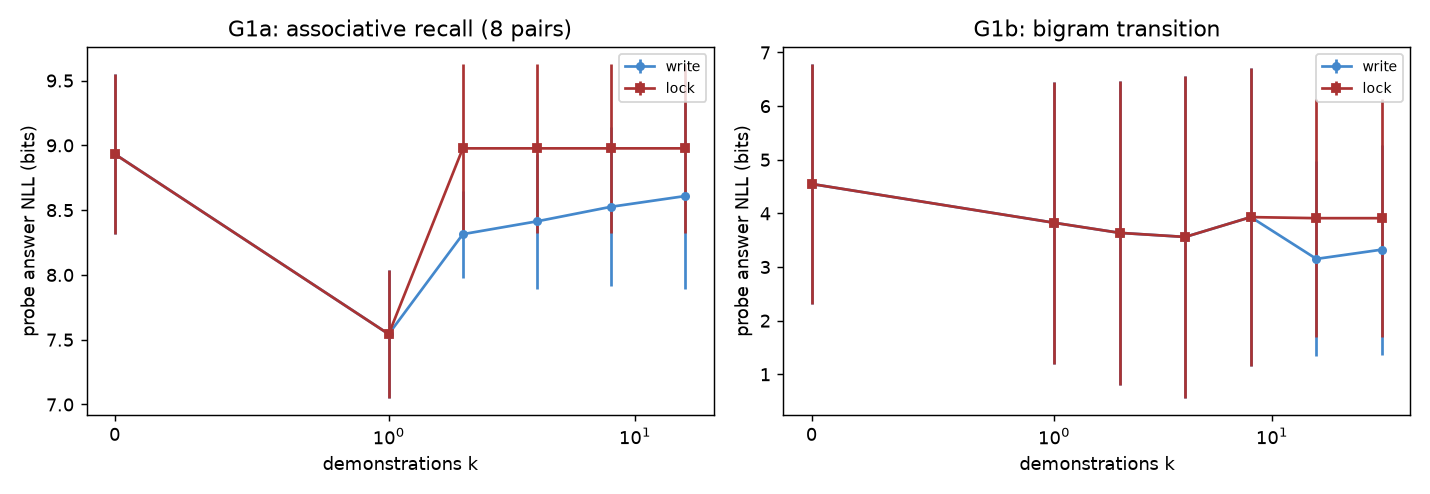
\includegraphics[width=\linewidth]{fig_g1_forward_learning.png}
\caption{G1a / G1b：前向学习曲线（$k$ 为演示次数）。联想任务上 write 曲线不随 $k$ 累积；
bigram 任务需要 $k\ge16$ 才出现跨 patch 效应，且置信区间极大。}
\label{fig:g1}
\end{figure}

\begin{figure}[H]
\centering
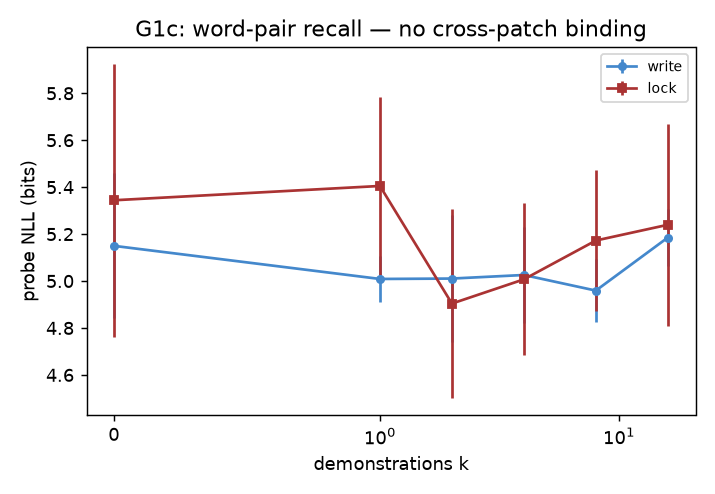
\includegraphics[width=0.62\linewidth]{fig_g1c_word_assoc.png}
\caption{G1c：把符号换成分布内高频词对后曲线依然全平（$\approx$ 首字节机会线），
排除「随机 ASCII 太 OOD」这一解释。}
\label{fig:g1c}
\end{figure}

\begin{figure}[H]
\centering
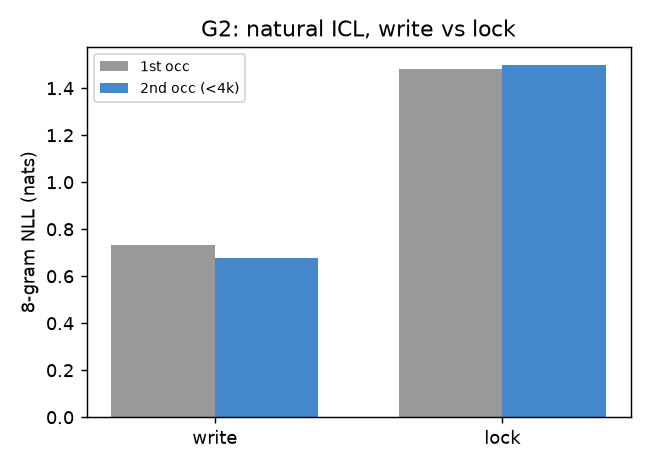
\includegraphics[width=0.55\linewidth]{fig_g2_natural_icl.png}
\caption{G2：自然语料 $8$-gram 的二次出现增益 $+0.054\nats$，且在 $\mathit{lock}$ 下消失——
说明该增益是写入依赖的、且量级很小。}
\label{fig:g2}
\end{figure}

\section{F 线与 H 线：未运行}\label{app:f-h}

F 线（训练动力学）需要重训，超出「只用现成权重」的范围：
BPTT 窗口扫描、永续 vs 文档边界重置、状态统计演化、\texttt{chunk\_size} 扫描、状态收敛时间。
H 线（任务级 demo：多会话一致性、长文档跨块一致性、代码跨文件一致性）依赖推理链冻结后再做。
两项都按 \S\ref{sec:f-line} 的优先级排序，本稿不给任何推测数值。


\clearpage  % 参考文献单独成页
\bibliographystyle{plainnat}
\bibliography{refs}

\end{document}
